% Created 2025-02-03 Mon 11:46
% Intended LaTeX compiler: pdflatex
\documentclass[presentation,smaller]{beamer}
\usepackage[utf8]{inputenc}
\usepackage[T1]{fontenc}
\usepackage{graphicx}
\usepackage{longtable}
\usepackage{wrapfig}
\usepackage{rotating}
\usepackage[normalem]{ulem}
\usepackage{amsmath}
\usepackage{amssymb}
\usepackage{capt-of}
\usepackage{hyperref}
\usetheme{Madrid}
\usefonttheme[onlymath]{serif}
\usecolortheme{default}
\AtBeginSection{\frame{\sectionpage}}
\newcommand{\ee}{\mathbf e}
\newcommand{\bb}{\mathbf b}
\newcommand{\RR}{\mathbf R}
\newcommand{\BB}{\mathbf B}
\newcommand{\CC}{\mathbf C}
\renewcommand{\SS}{\mathbf S}
\newcommand{\UU}{\mathbf U}
\newcommand{\VV}{\mathbf V}
\newcommand{\Lag}{\mathcal L}
\newcommand{\la}{\lambda}
\newcommand{\bla}{\boldsymbol{\lambda}}
\newcommand{\bone}{\mathbf{1}}
\newcommand{\bzero}{\mathbf{0}}
\newcommand{\yy}{\mathbf{y}}
\newcommand{\rr}{\mathbf{r}}
\newcommand{\cc}{\mathbf{c}}
\renewcommand{\AA}{\mathbf{A}}
\newcommand{\xx}{\mathbf{x}}
\newcommand{\uu}{\mathbf{u}}
\newcommand{\vv}{\mathbf{v}}
\newcommand{\red}[1]{{\color{red}#1}}
\renewcommand{\bold}[1]{\textbf{#1}}
\DeclareMathOperator{\var}{var}
\DeclareMathOperator{\cov}{cov}
  

\usetheme{default}
\author{Sina Tootoonian}
\date{}
\title{Dimensionality Reduction using\newline Principal Component Analysis}
\title[Dimensionality Reduction using PCA]{Dimensionality Reduction using\newline Principal Component Analysis}
\hypersetup{
 pdfauthor={Sina Tootoonian},
 pdftitle={Dimensionality Reduction using\newline Principal Component Analysis},
 pdfkeywords={},
 pdfsubject={},
 pdfcreator={Emacs 28.2 (Org mode 9.5.5)}, 
 pdflang={English}}
\begin{document}

\maketitle
\begin{frame}{Outline}
\tableofcontents
\end{frame}

\section{Motivation}
\label{sec:org14c7e8b}
\begin{frame}[label={sec:org4c7cf05}]{Neuroscience data arrive high dimensional}
\begin{figure}[htbp]
\centering
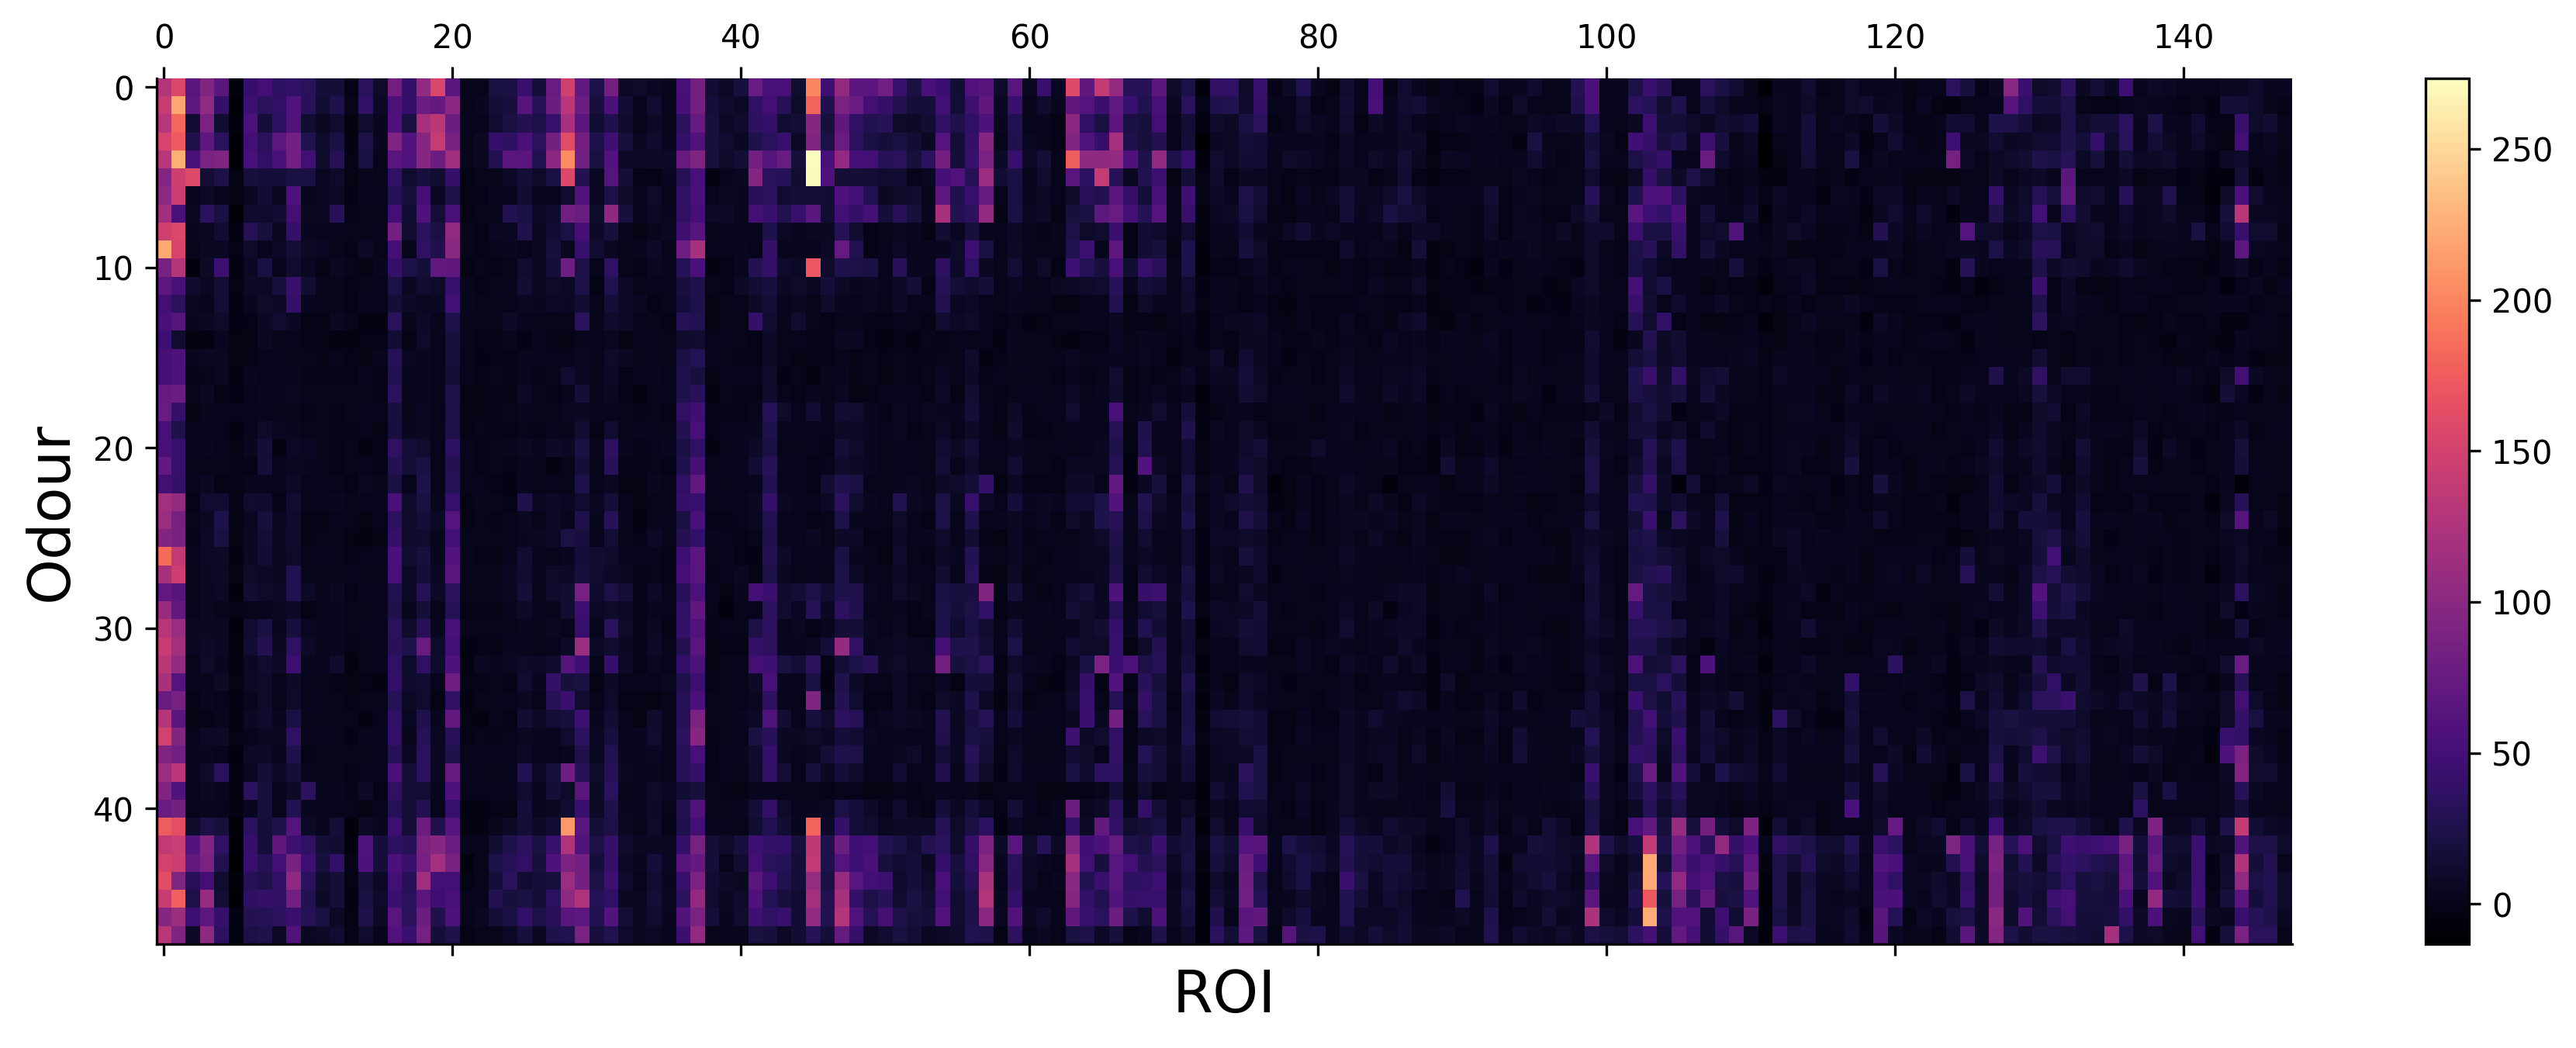
\includegraphics[width=1.0\textwidth]{figures/heatmap.png}
\caption{Response of 150 olfactory glomeruli to 48 odours (Tobias Ackels)}
\end{figure}
\end{frame}
\begin{frame}[label={sec:org2f4f994}]{Visualization requires 2-3 dimensions}
\begin{figure}[htbp]
\centering
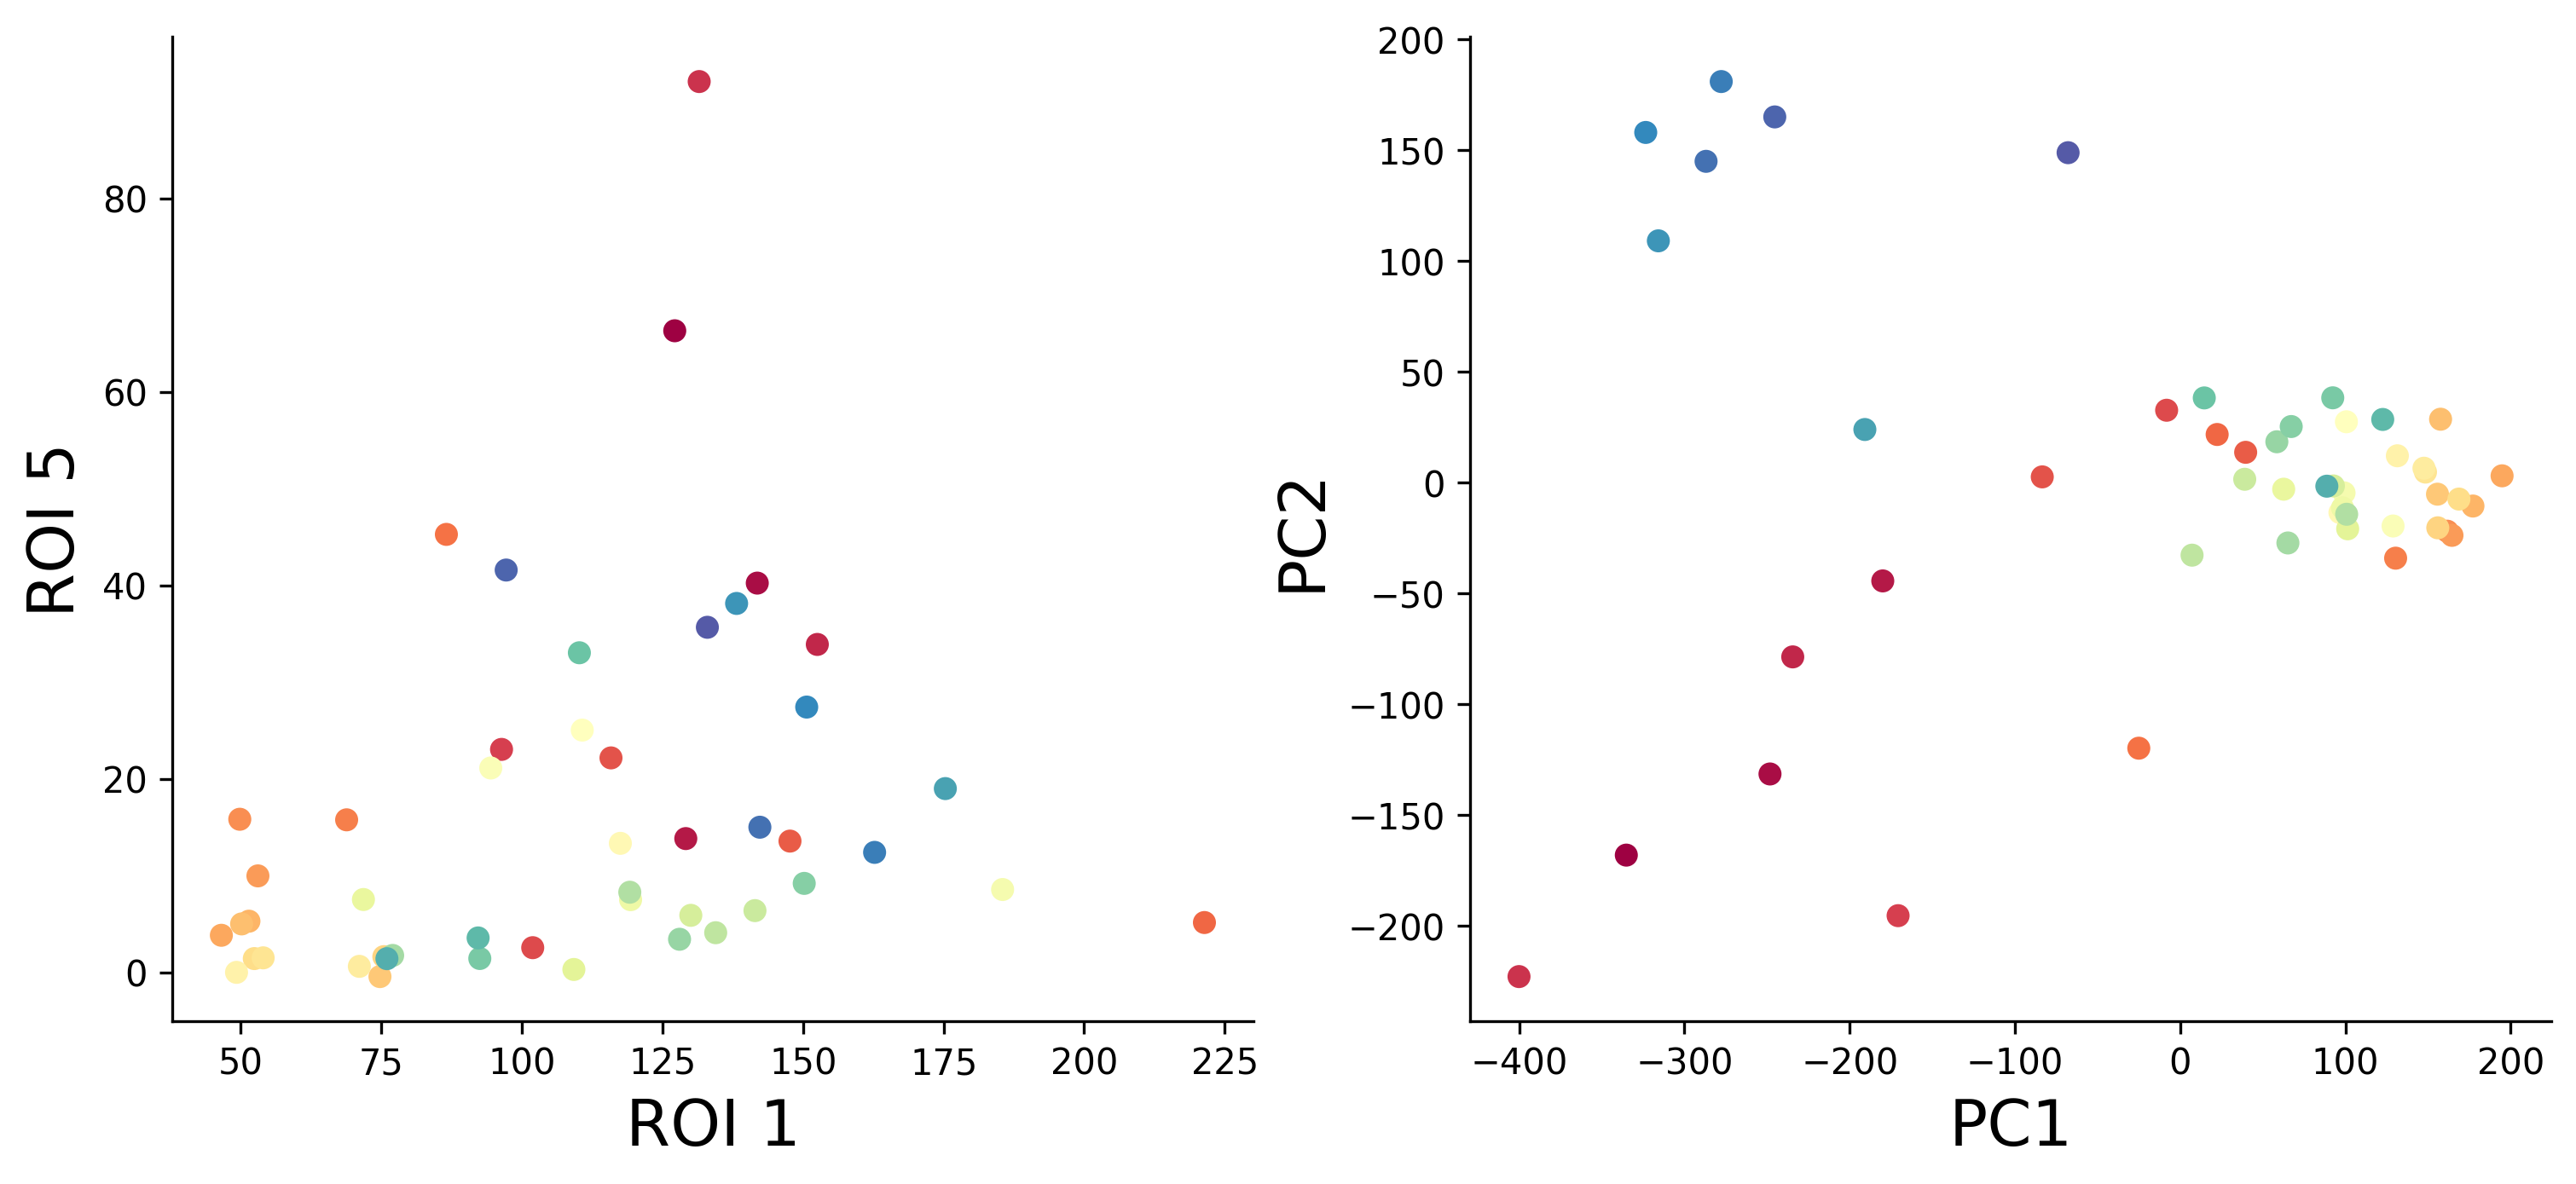
\includegraphics[width=1.0\textwidth]{figures/PCA.png}
\caption{Odour responses of two ROIs, vs. two principal components.}
\end{figure}
\end{frame}
\begin{frame}[label={sec:org1f8b705}]{High-D data can be embeddings of low-D manifolds}
\begin{figure}[htbp]
\centering
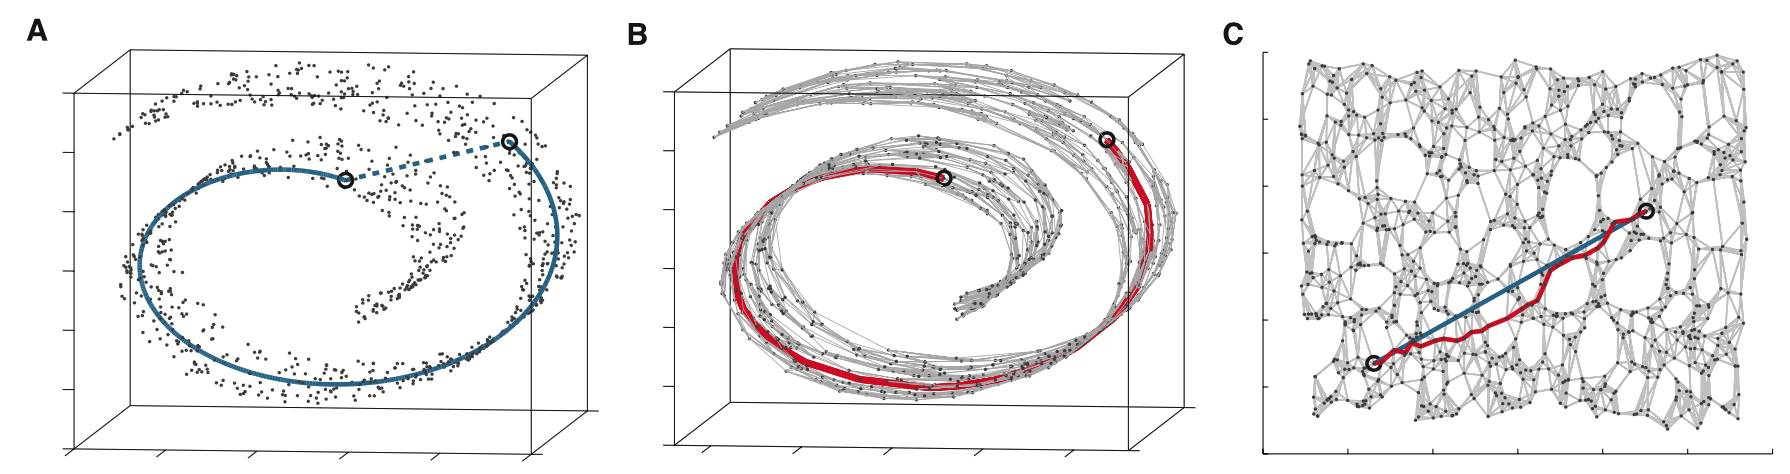
\includegraphics[width=1.0\textwidth]{figures/swiss_roll.png}
\caption{`Swiss roll' dataset from Tenenbaum et al. 2000.}
\end{figure}
\end{frame}
\begin{frame}[label={sec:orgd12f4ef}]{Data compression / approximation / denoising}
\begin{figure}[htbp]
\centering
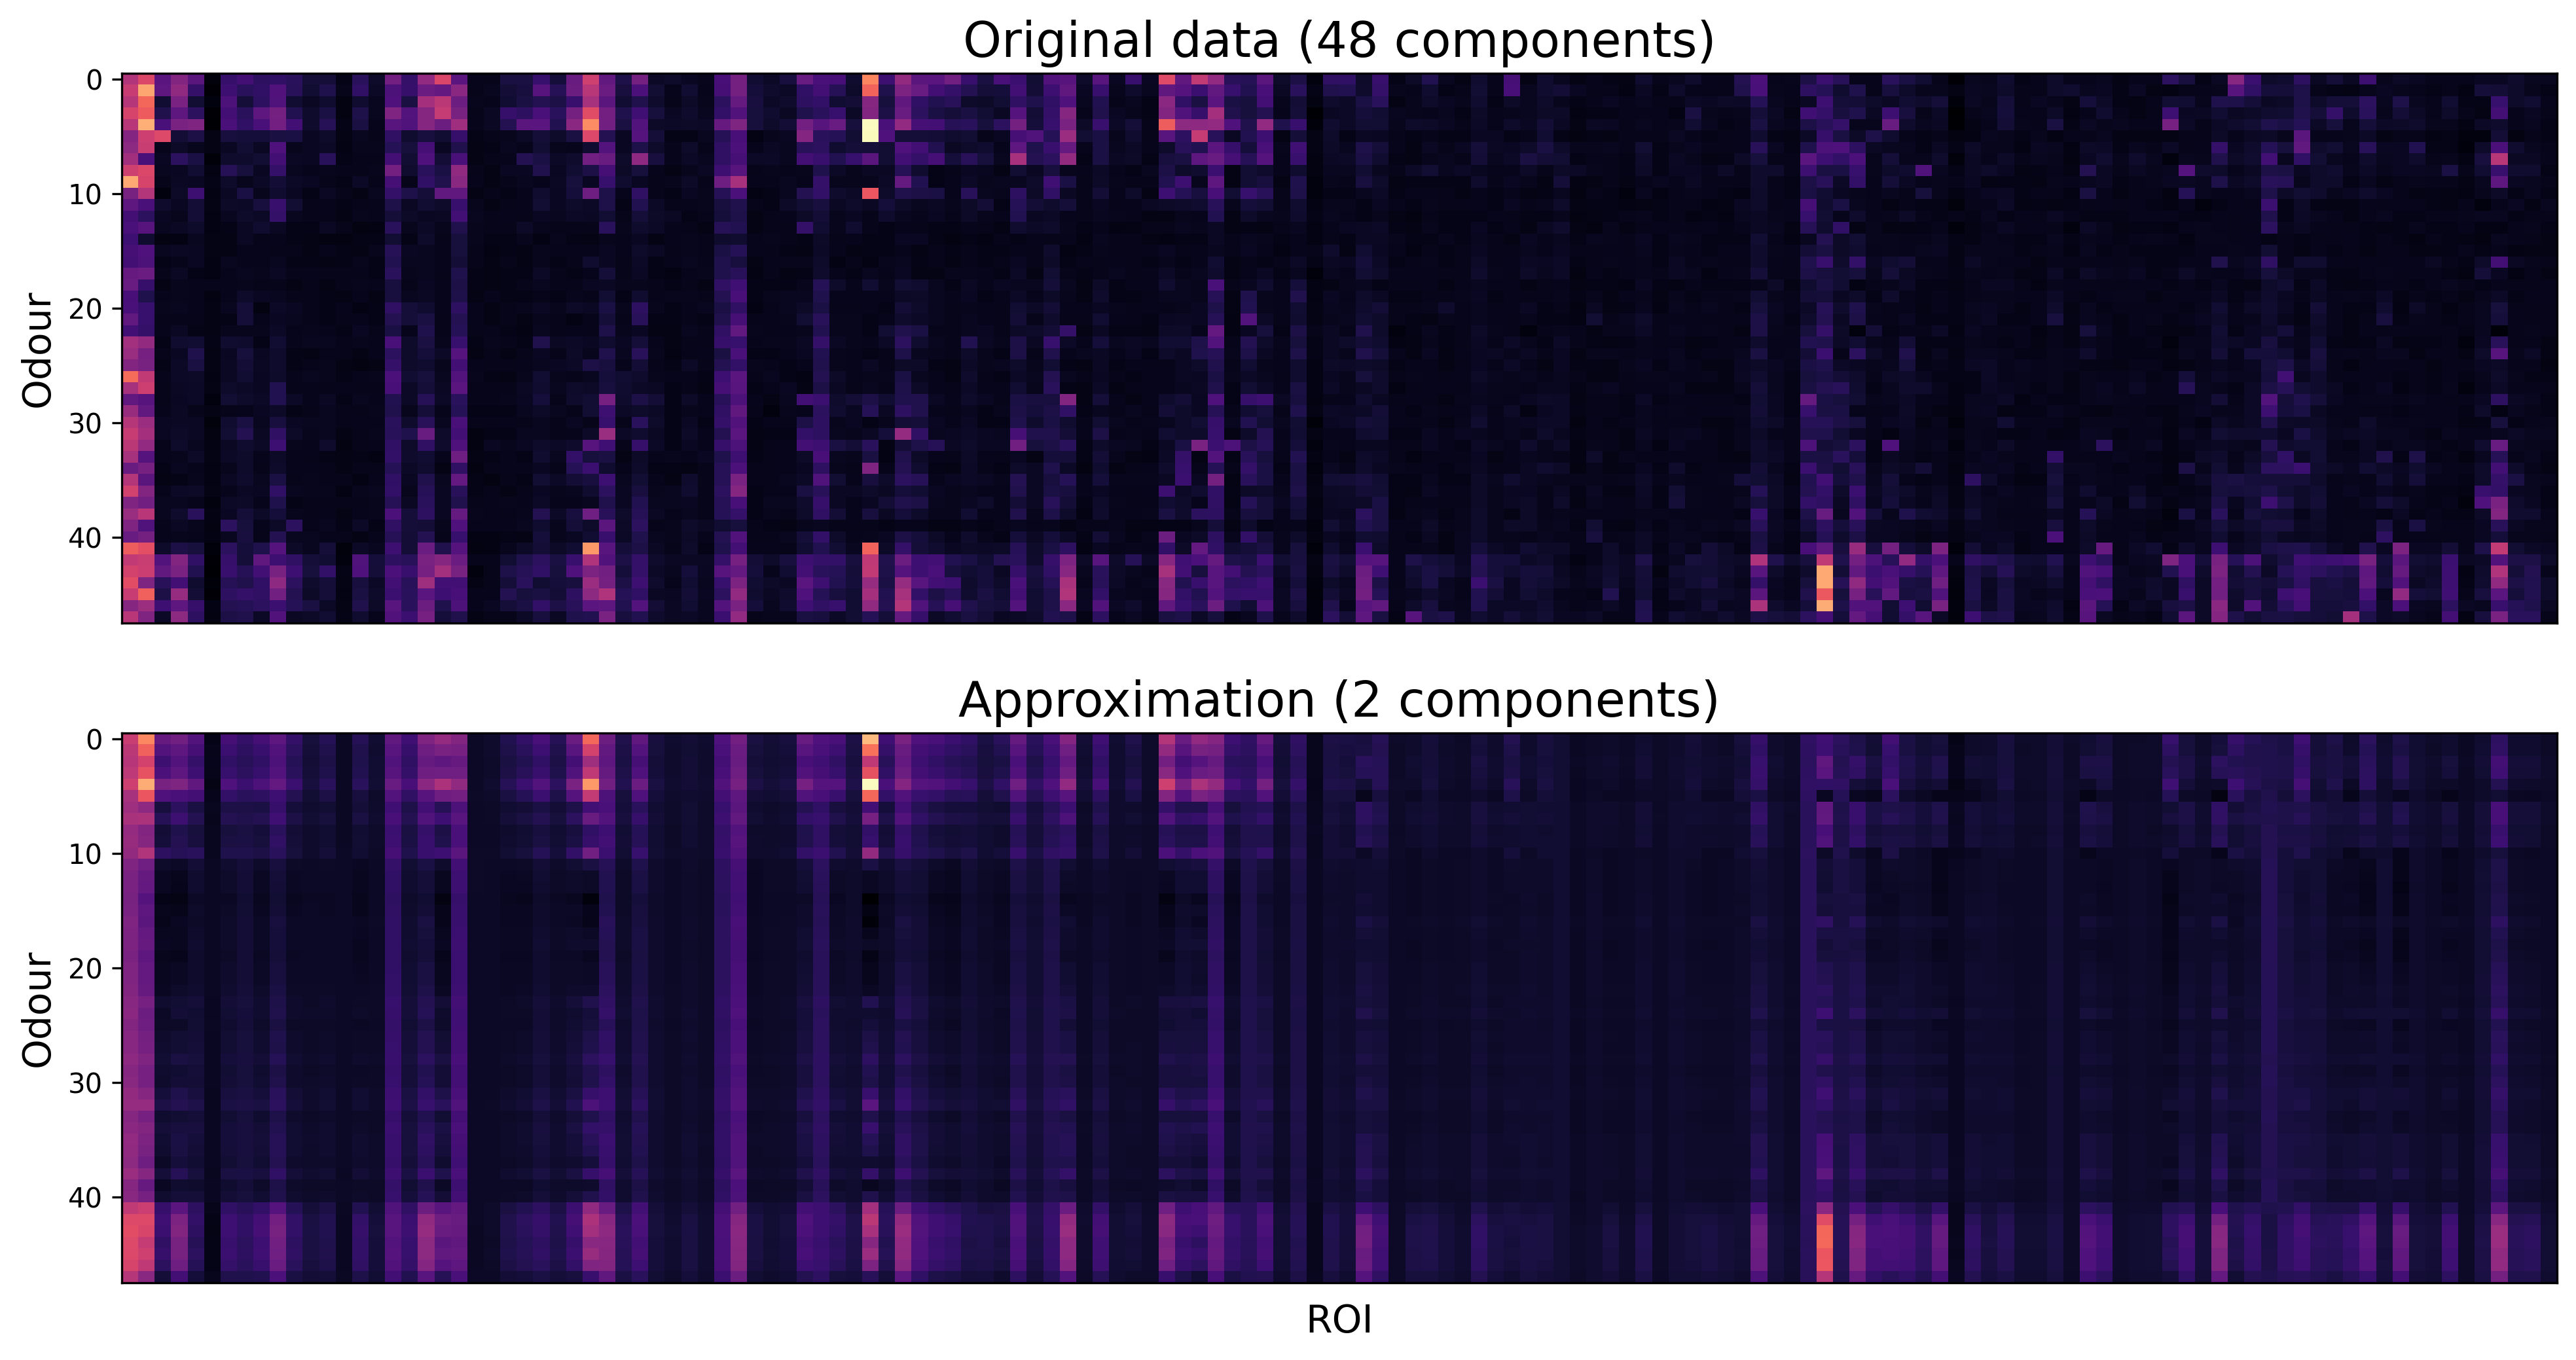
\includegraphics[width=1.0\textwidth]{figures/rank2_approx.png}
\caption{Raw odour responses and 2-component approximation.}
\end{figure}
\end{frame}
\begin{frame}[label={sec:org9808c67}]{Key idea behind PCA}
   \begin{center}
\Large
Find \bold{directions} in data space that \bold{maximize} \bold{variance}.
\end{center}

\vspace{1cm}
\begin{itemize}
\item What do we mean by \emph{directions}?
\item What do we mean by \emph{variance}?
\item Why is \emph{maximizing} a good idea?
\end{itemize}
\end{frame}
\begin{frame}[label={sec:org0906655}]{Key idea behind PCA}
\begin{figure}[htbp]
\centering
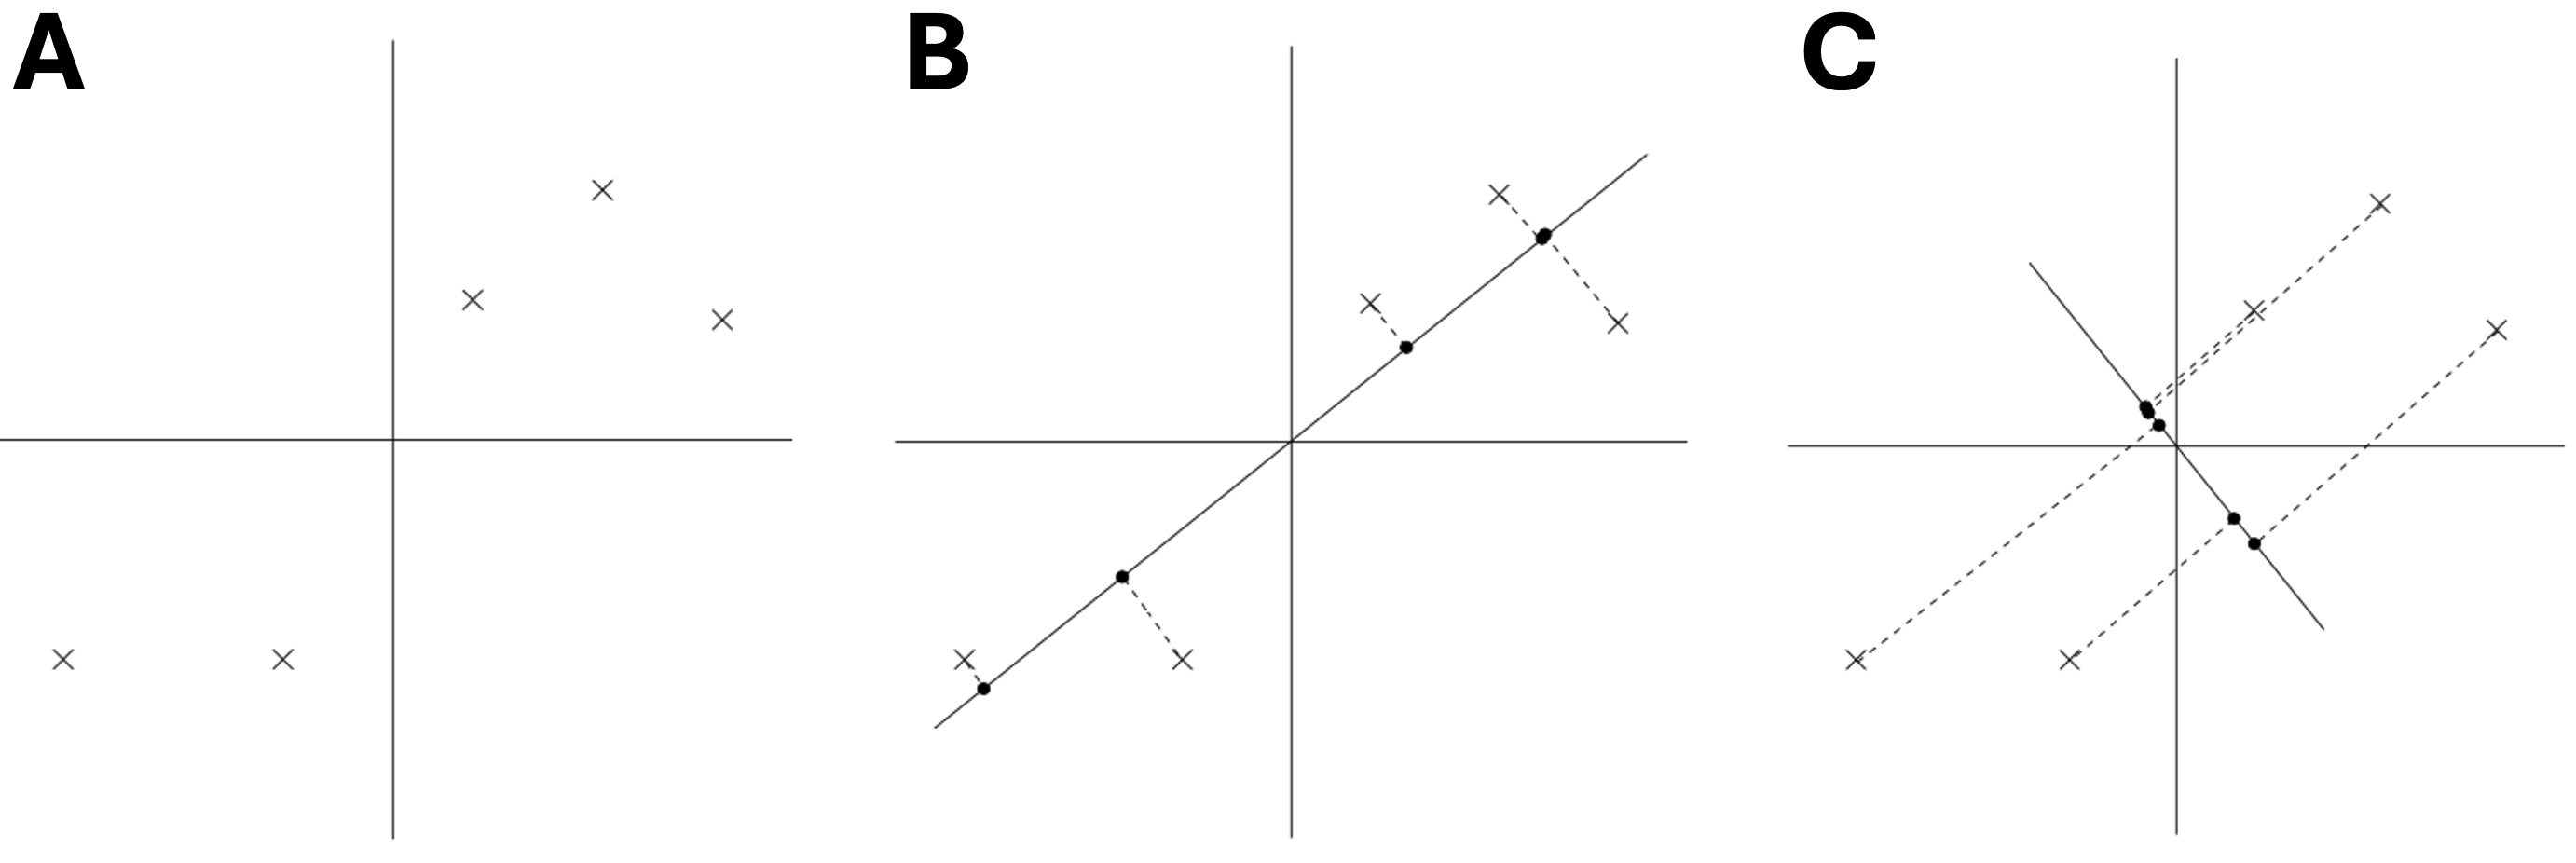
\includegraphics[width=1.0\textwidth]{figures/example_proj.png}
\caption{Projecting data (A) along directions that capture much (B) or little (C) variance. From CS 229.}
\end{figure}
\end{frame}
\begin{frame}[label={sec:org4666287}]{Outline}
\begin{enumerate}
\item Single neurons
\begin{itemize}
\item Single neurons as coordinates.
\item Variance of single neurons, covariance of populations of neurons.
\item Variance of single neurons as covariance along standard coordinates.
\end{itemize}
\item Pseudo-neurons
\begin{itemize}
\item Other orthonormal coordinates define \bold{pseudo-neurons}.
\item Variance of pseudo-neurons as covariance along their coordinates.
\item PCA = finding pseudo-neurons with maximum variance.
\end{itemize}
\item PCA by Singular Value Decomposition
\begin{itemize}
\item Some facts about matrices.
\item Singular Value Decomposition (SVD).
\item Maximum variance directions from SVD.
\end{itemize}
\item Application to neural responses.
\item Adjacent approaches: Kernel PCA, CCA, LDA.
\end{enumerate}
\end{frame}
\section{Variance of Single Neurons}
\label{sec:org5c3f6ee}
\begin{frame}[label={sec:org9ff128c}]{Notions of dimensionality}
\begin{center}
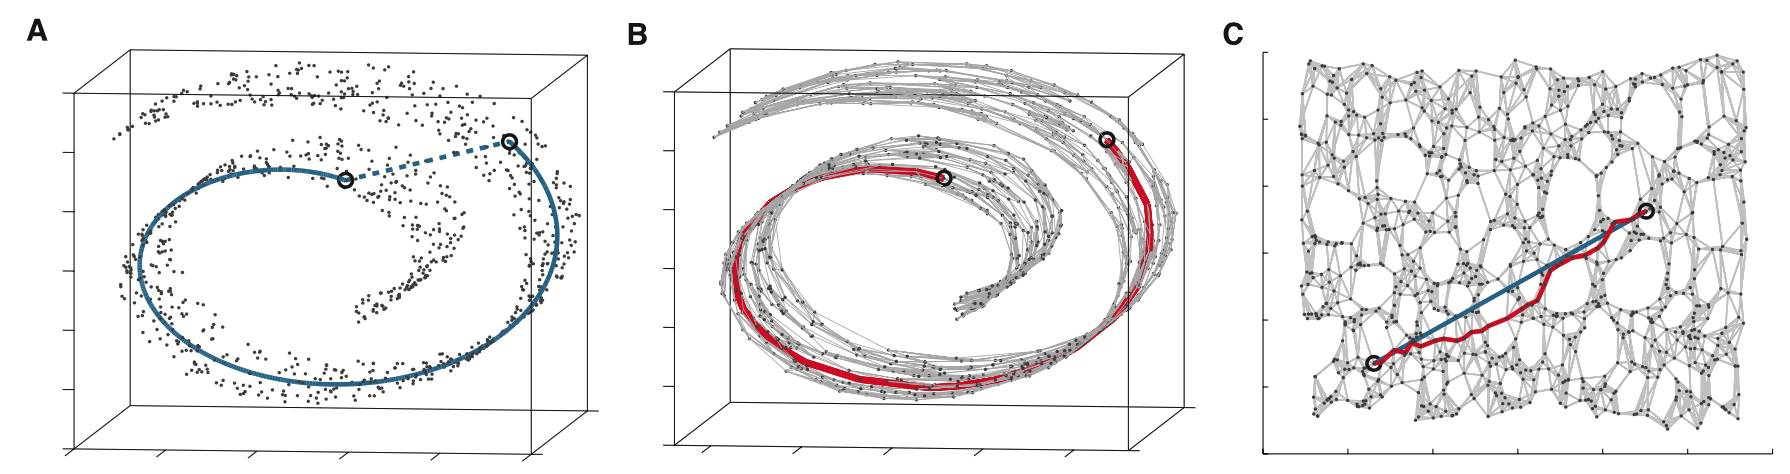
\includegraphics[width=1.0\textwidth]{figures/swiss_roll.png}
\end{center}  
\begin{itemize}
\item Extrinsic dimension
\item Intrinsic dimension
\begin{itemize}
\item Lower because of correlations in the data
\end{itemize}
\item PCA: Find the intrinsic, \bold{linear} dimension
\end{itemize}
\end{frame}
\begin{frame}[label={sec:orgf3f48a8}]{The importance of coordinate systems}
\begin{itemize}
\item Laws of physics don't depend on coordinates.
\item Laws of neuroscience depends on having the right coordiantes
\begin{itemize}
\item Usually not the ones your data is recorded in.
\end{itemize}
\item PCA finds coordinates that are \bold{matched to the data}.
\end{itemize}
\begin{center}
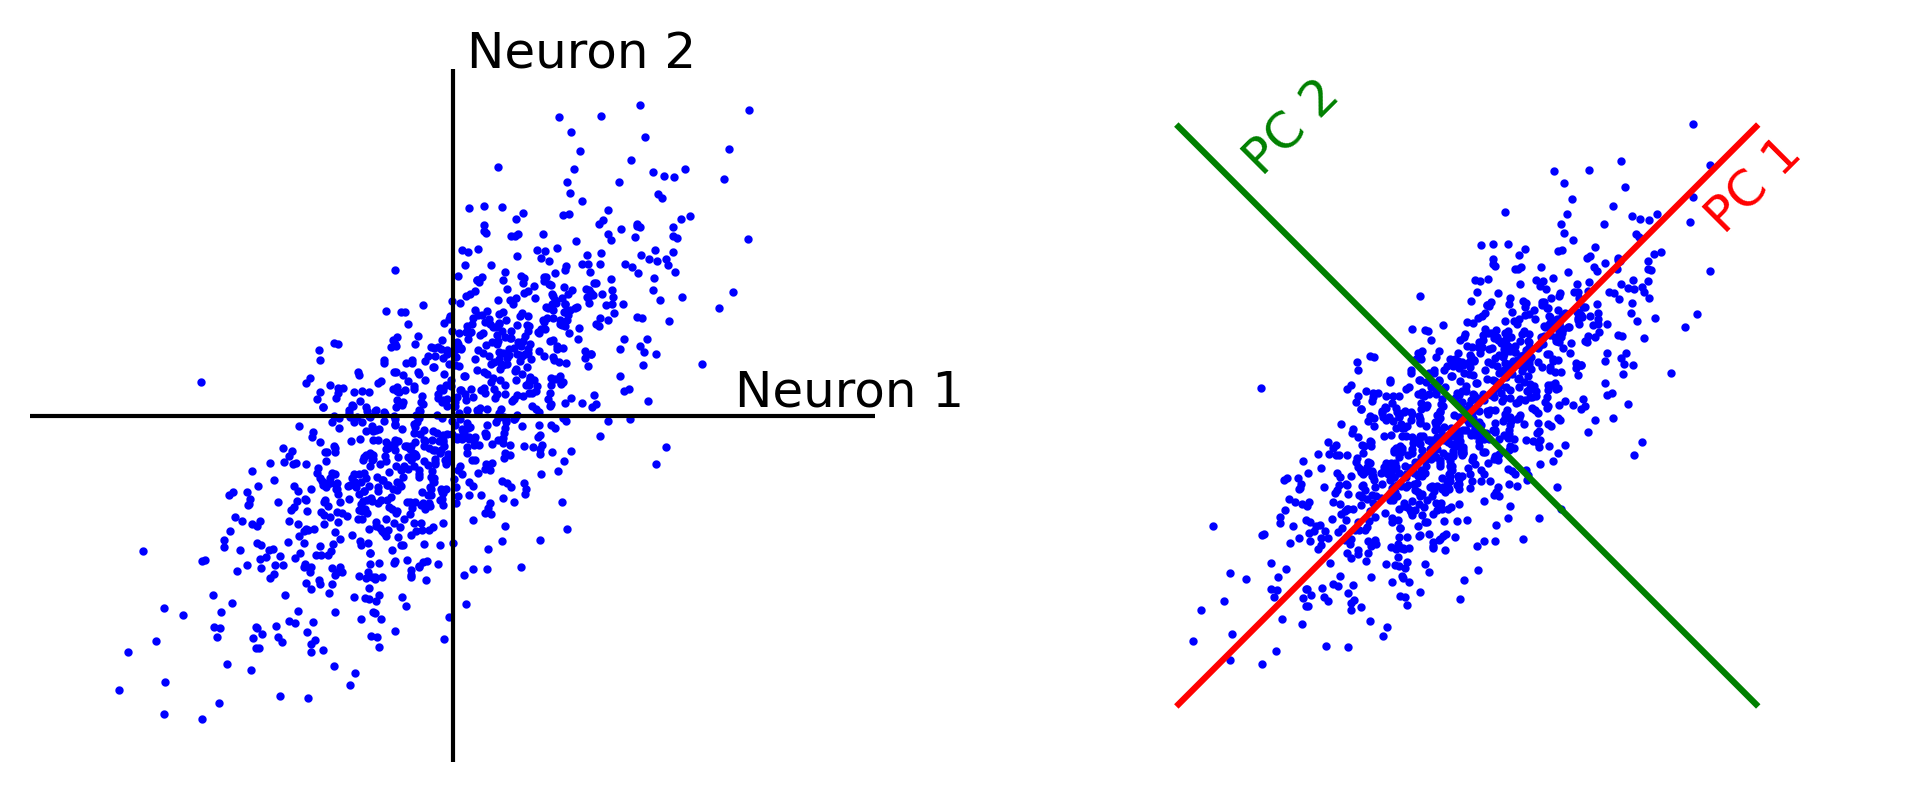
\includegraphics[width=1.0\textwidth]{figures/pca_illustration.png}
\end{center}  
\end{frame}
\begin{frame}[label={sec:org6f99866}]{Standard coordinates}
\begin{center}
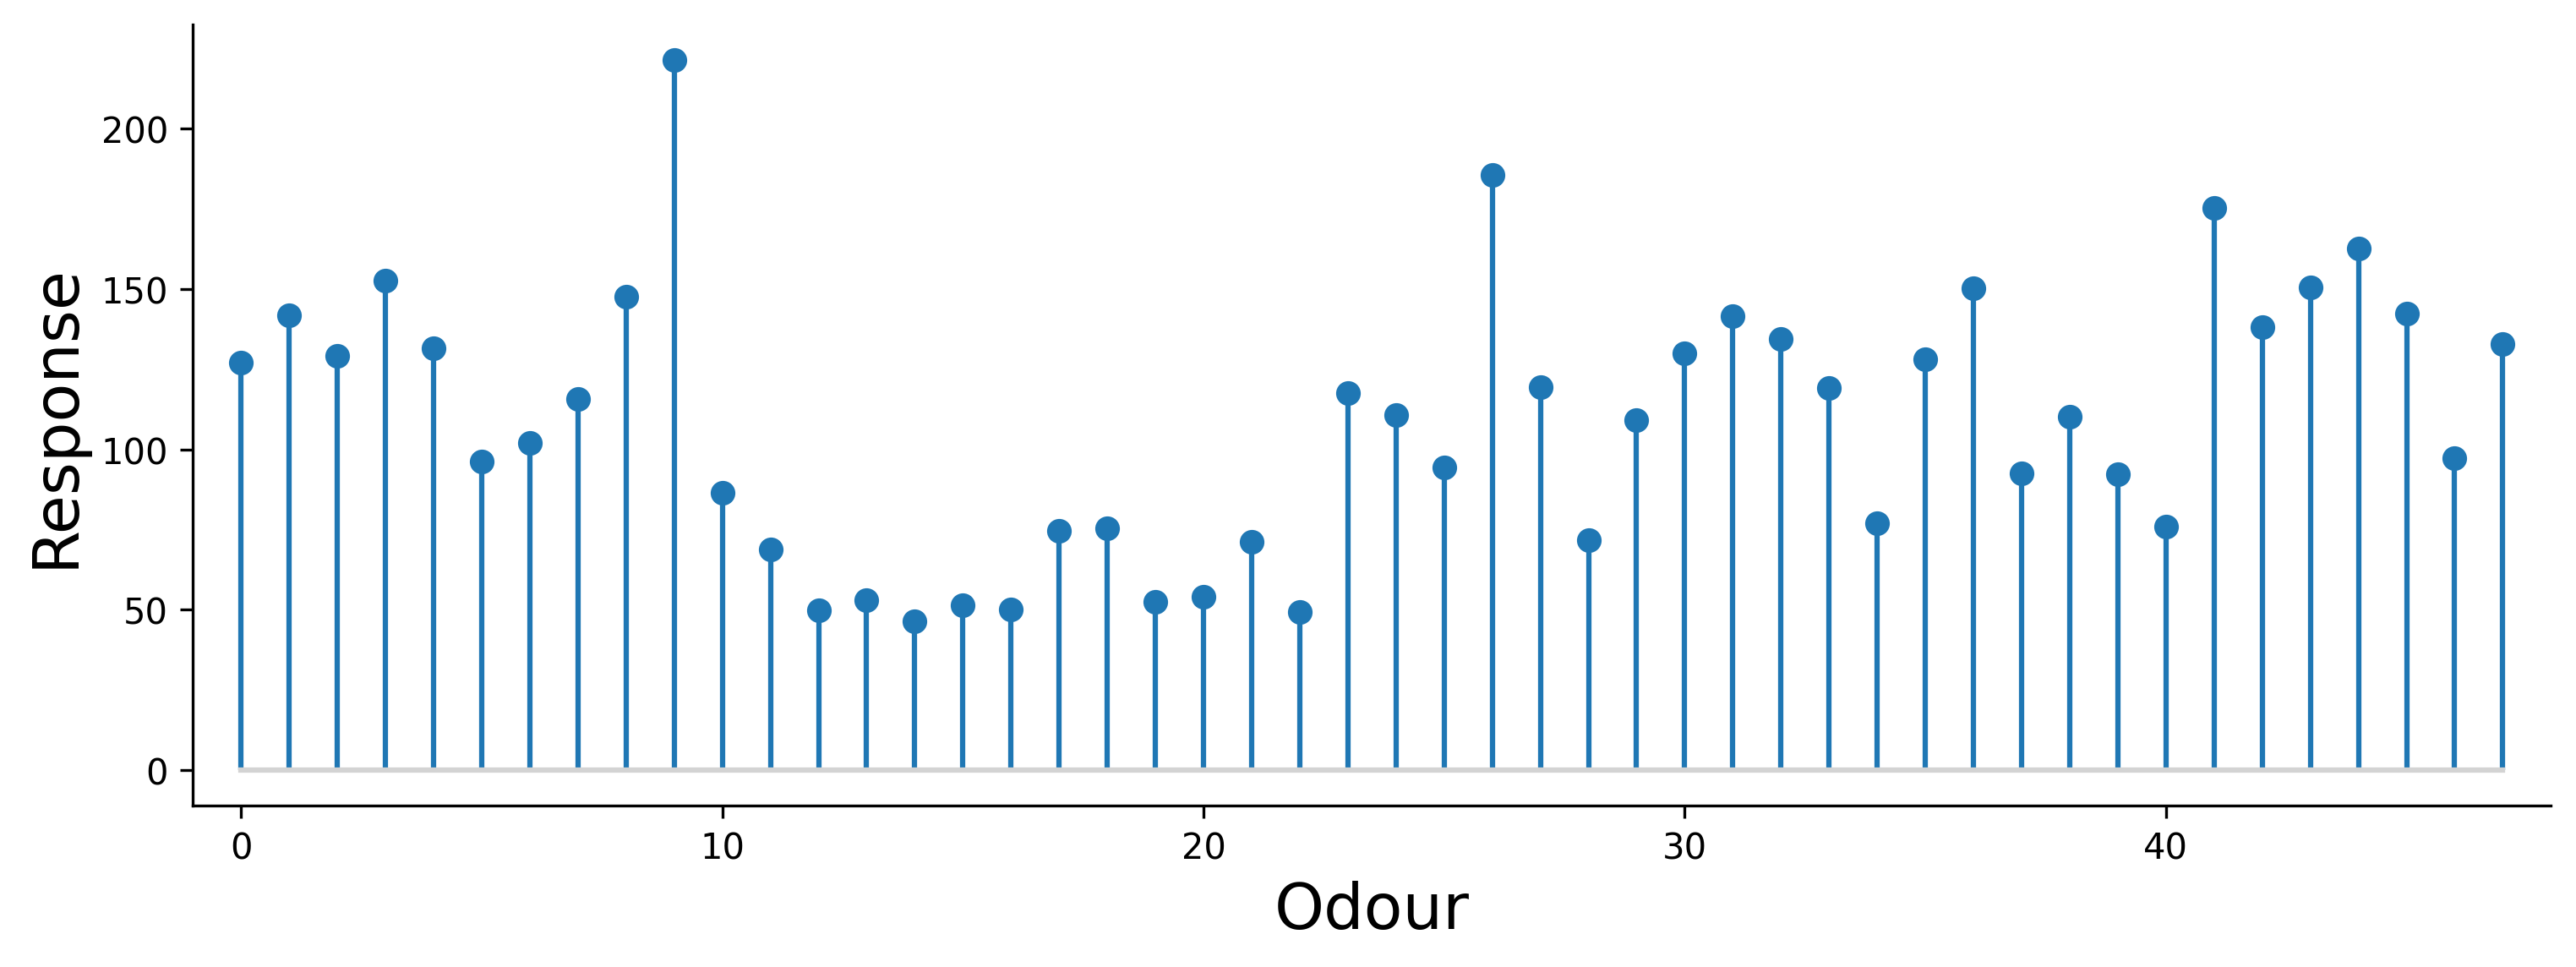
\includegraphics[width=1.0\textwidth]{figures/one_odour_response.png}
\end{center}
\begin{itemize}
\item Notice implicit coordinates:
\begin{align*}
\xx &= [x_1, x_2, \dots ] \\
&=x_1 \ee_1 + x_2 \ee_2 + \dots
\end{align*}
\item Each coordinate \(\ee_1\), \(\ee_2\) corresponds to unit activity of one neuron.
\end{itemize}
\end{frame}
\begin{frame}[label={sec:orgf3bac90}]{Coordinates are orthonormal}
\vspace{-0.25cm}
\begin{center}
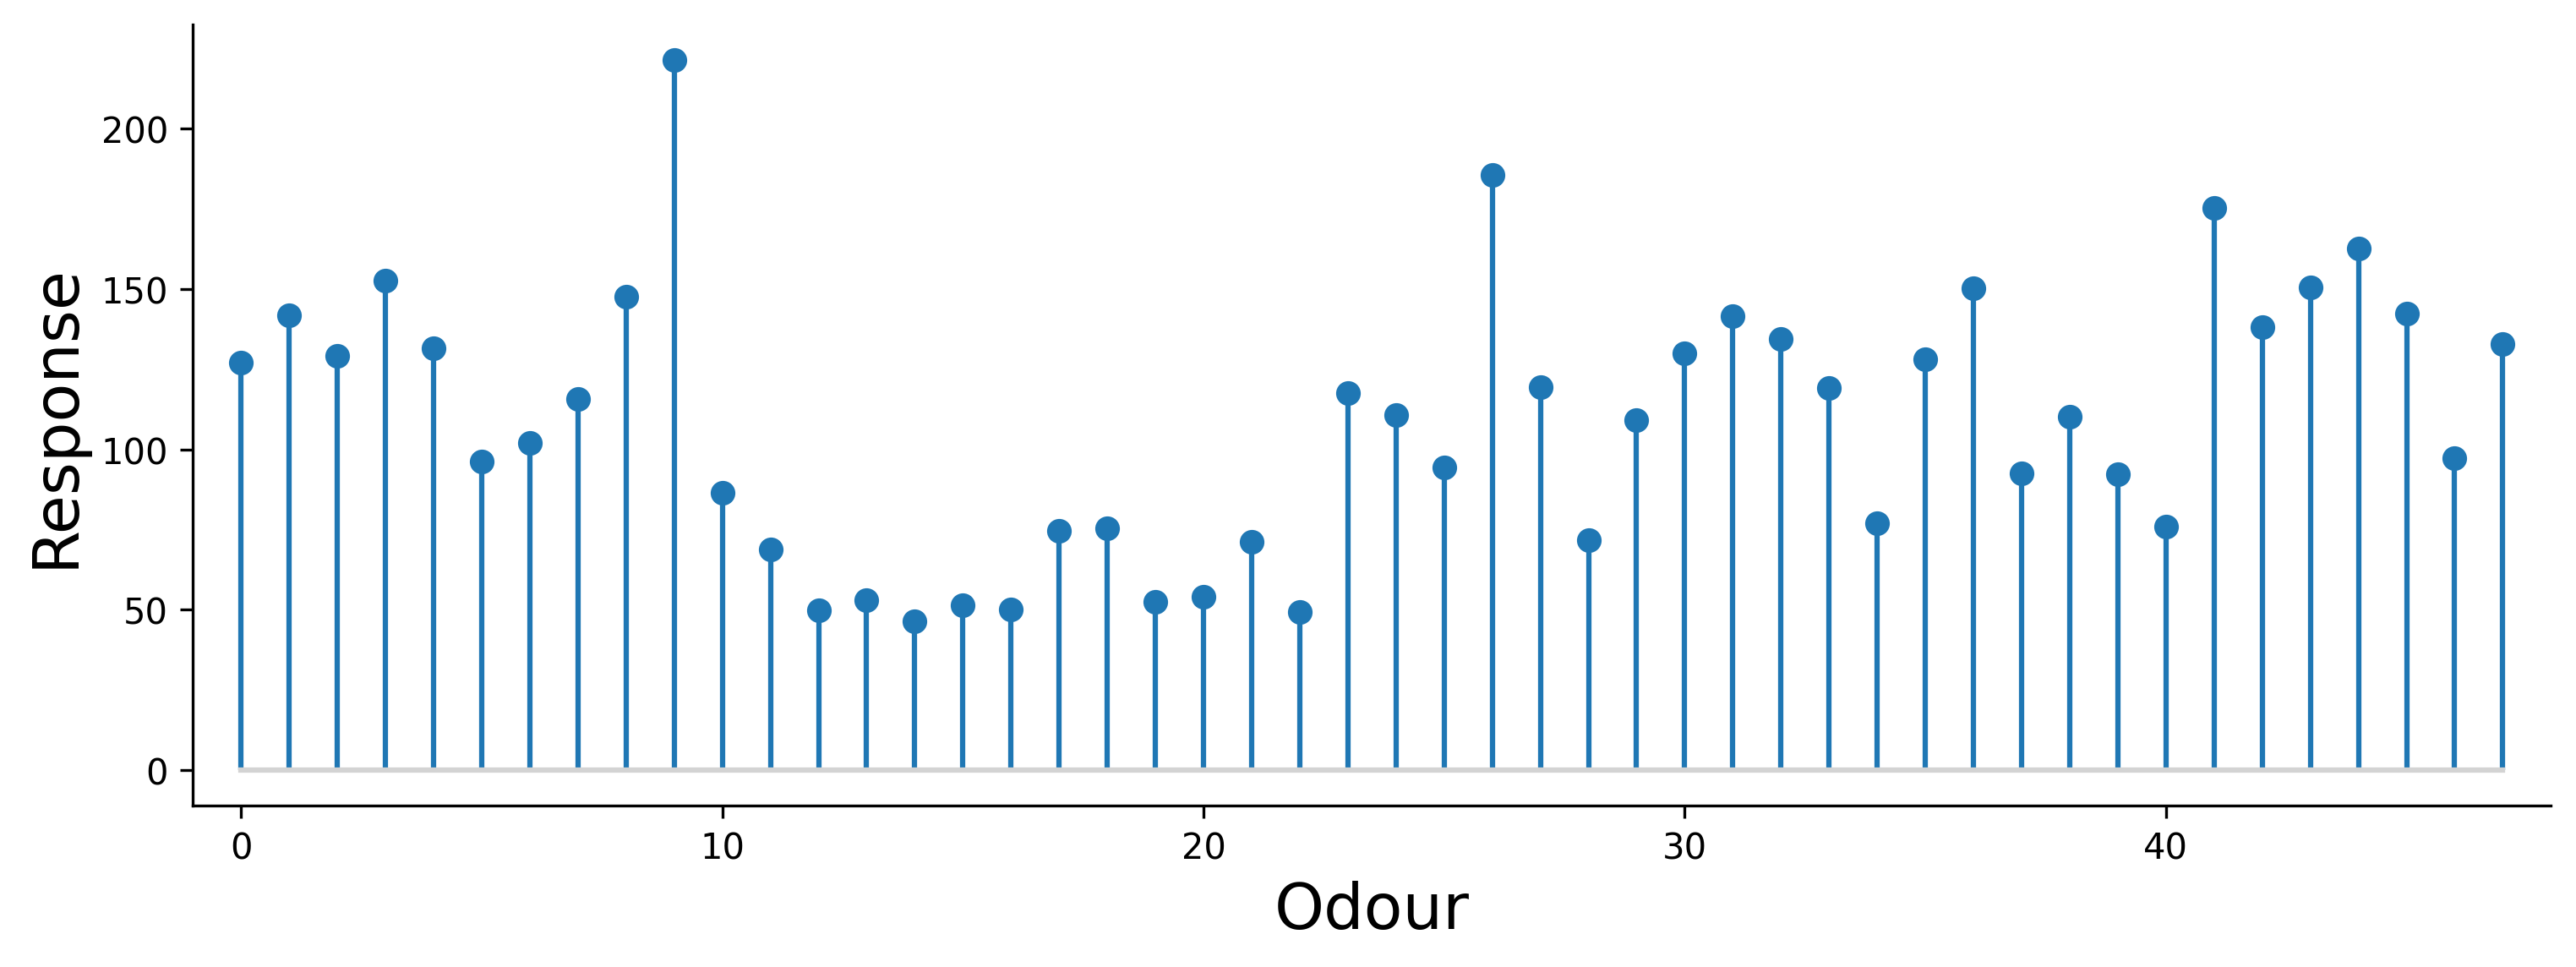
\includegraphics[width=1.0\textwidth]{figures/one_odour_response.png}
\end{center}
$$\xx = x_1 \ee_1 + x_2 \ee_2 \dots$$
\vspace{-0.25cm}
\begin{itemize}
\item The coordinate system \(\{ \ee_1, \ee_2, \dots \}\) is:
\begin{itemize}
\item Complete: We can represent any activity vector in it.
\item Ortho\ldots{}  $$ \ee_1^T\ee_2  = 0, \dots $$
\item \ldots{}normal $$\ee_1^T \ee_1  = 1, \quad \ee_2^T\ee_2  = 1, \dots$$
\end{itemize}
\end{itemize}
\end{frame}
\begin{frame}[label={sec:org62c26cd}]{Extracting single unit responses by projection}
\begin{center}
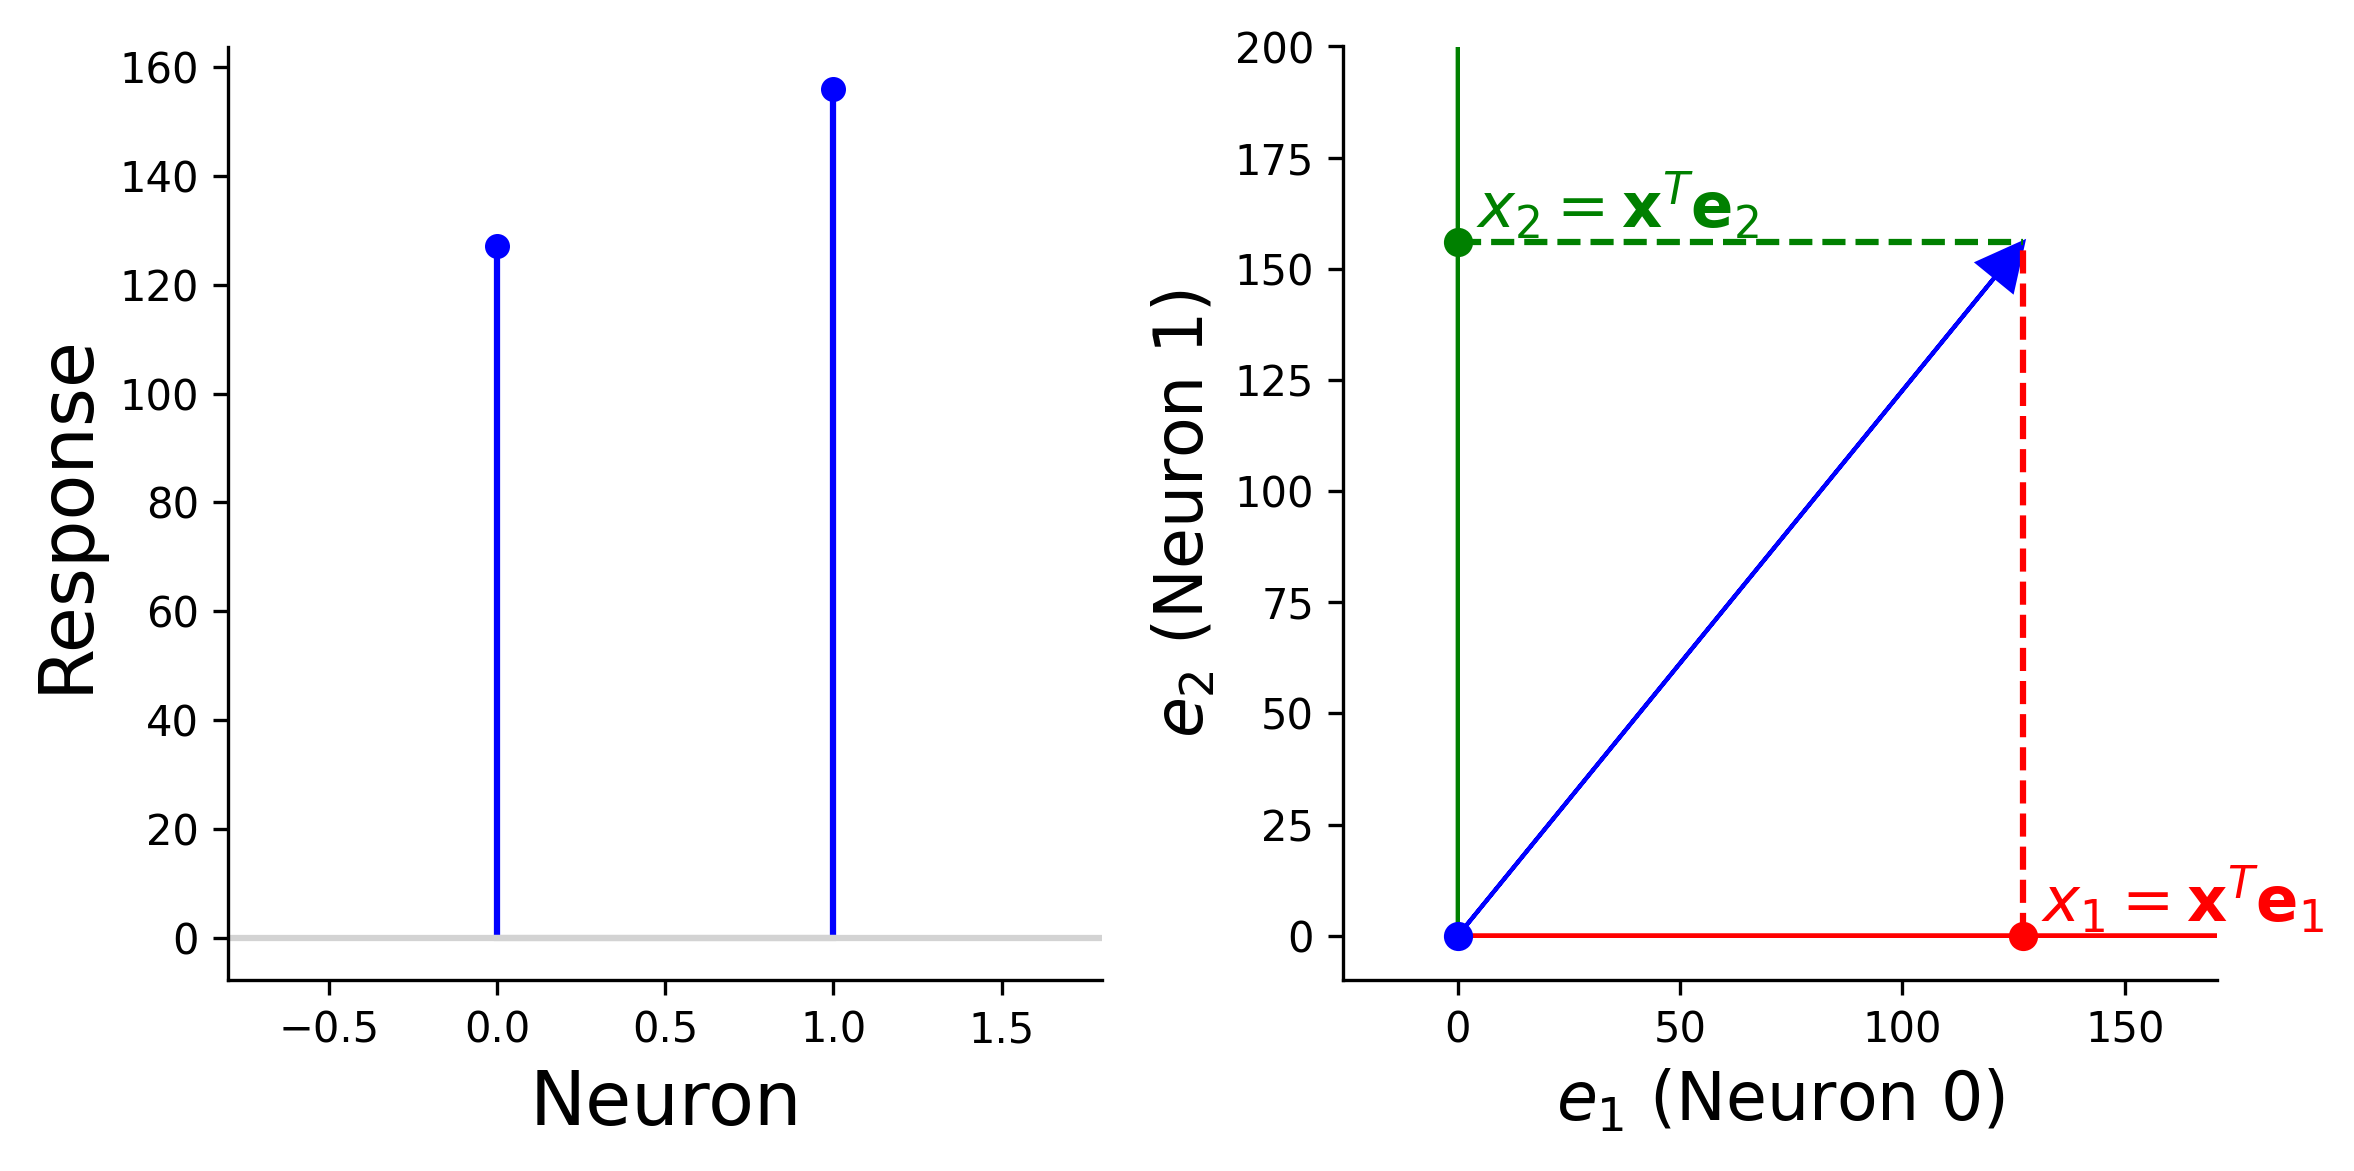
\includegraphics[width=1.0\textwidth]{figures/projections.png}
\end{center}
  $$ x_1 = \xx^T \ee_1 = \ee_1^T \xx $$
\end{frame}
\begin{frame}[label={sec:orgfe18c5e}]{Different ways of summarizing activity}
\begin{center}
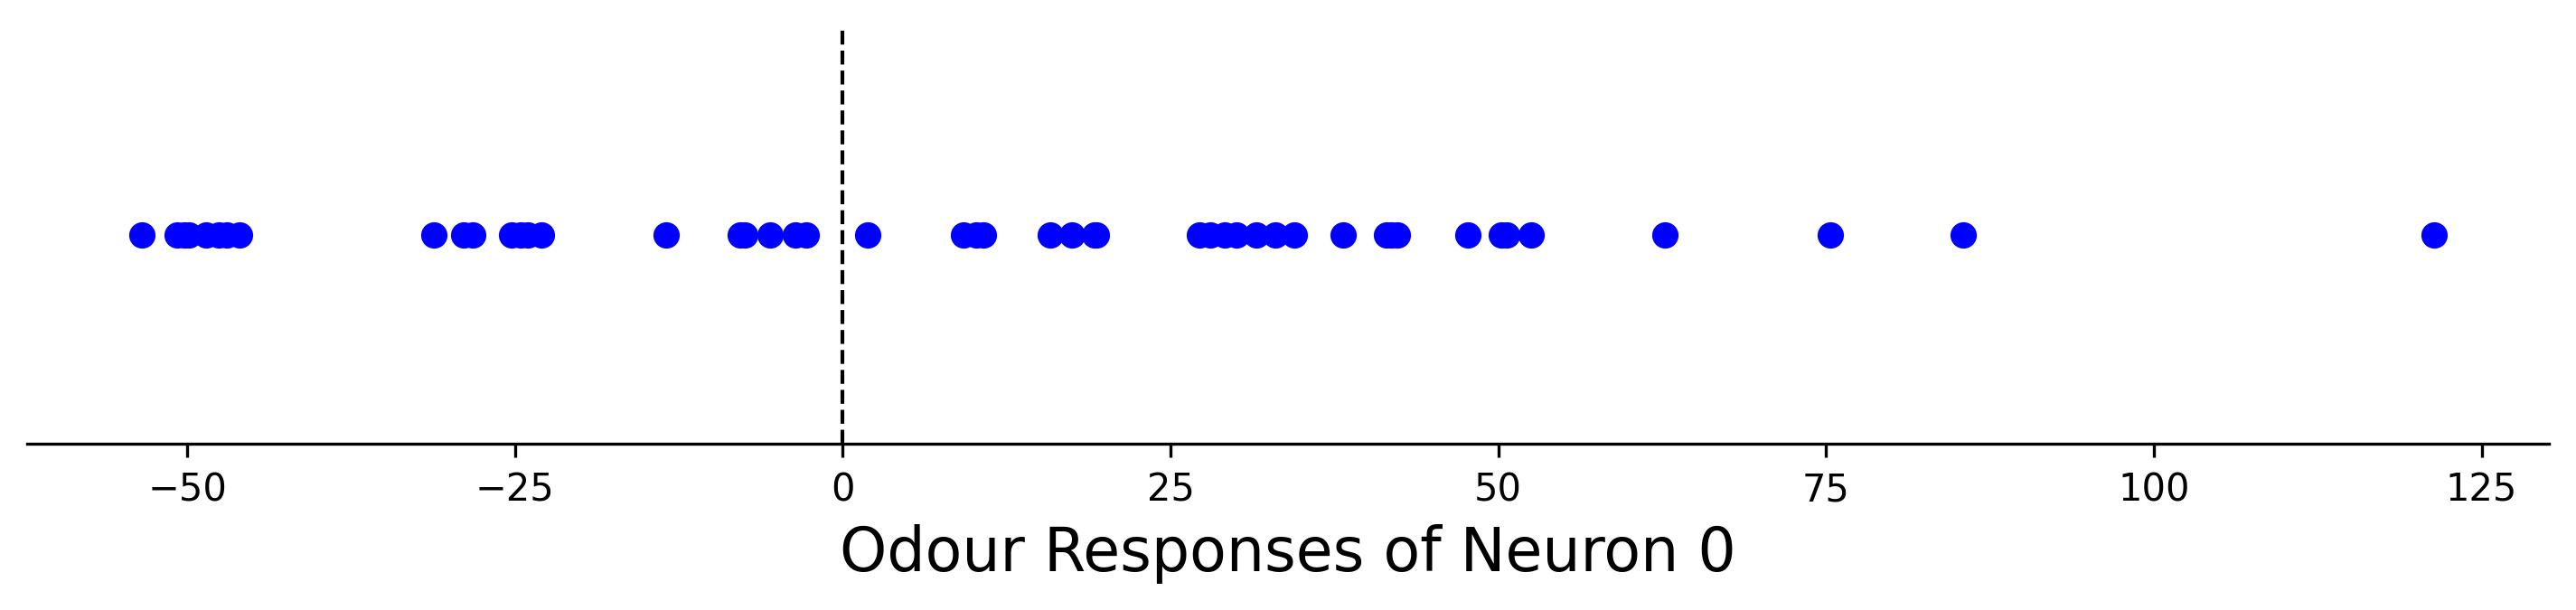
\includegraphics[width=1.0\textwidth]{figures/neuron0.png}
\end{center}  
\begin{itemize}
\item Mean?
$$ \overline{x}_1 = {1 \over \text{\# stimuli}} \sum_{\color{red}\mu\color{black}} x_{1,\color{red}\mu\color{black}} = \langle x_{1,\mu} \rangle.$$
\item Absolute value? $$\overline{|x_1|} = \langle |x_{1,\mu}| \rangle$$
\item Absolute value relative to mean?
$$ \overline{|x_1 - \overline{x}_1|} = \langle |x_{1,\mu} - \overline{x}_1 | \rangle.$$
\item Squared value?
$$ \overline{x^2_1} = \langle x^2_{1,\mu} \rangle$$
\end{itemize}
\end{frame}
\begin{frame}[label={sec:orgc952005}]{Variance of a single neuron}
$$ \var(x_1) = \langle (x_{1,\mu} - \overline{x}_1)^2 \rangle.$$
\begin{itemize}
\item Average energy relative to the mean
\item Mathematically tractable \color{green}\(\checkmark\)\color{black}
\item Susceptible to outliers \color{red}\textbf{X}\color{black}
\end{itemize}
\begin{center}
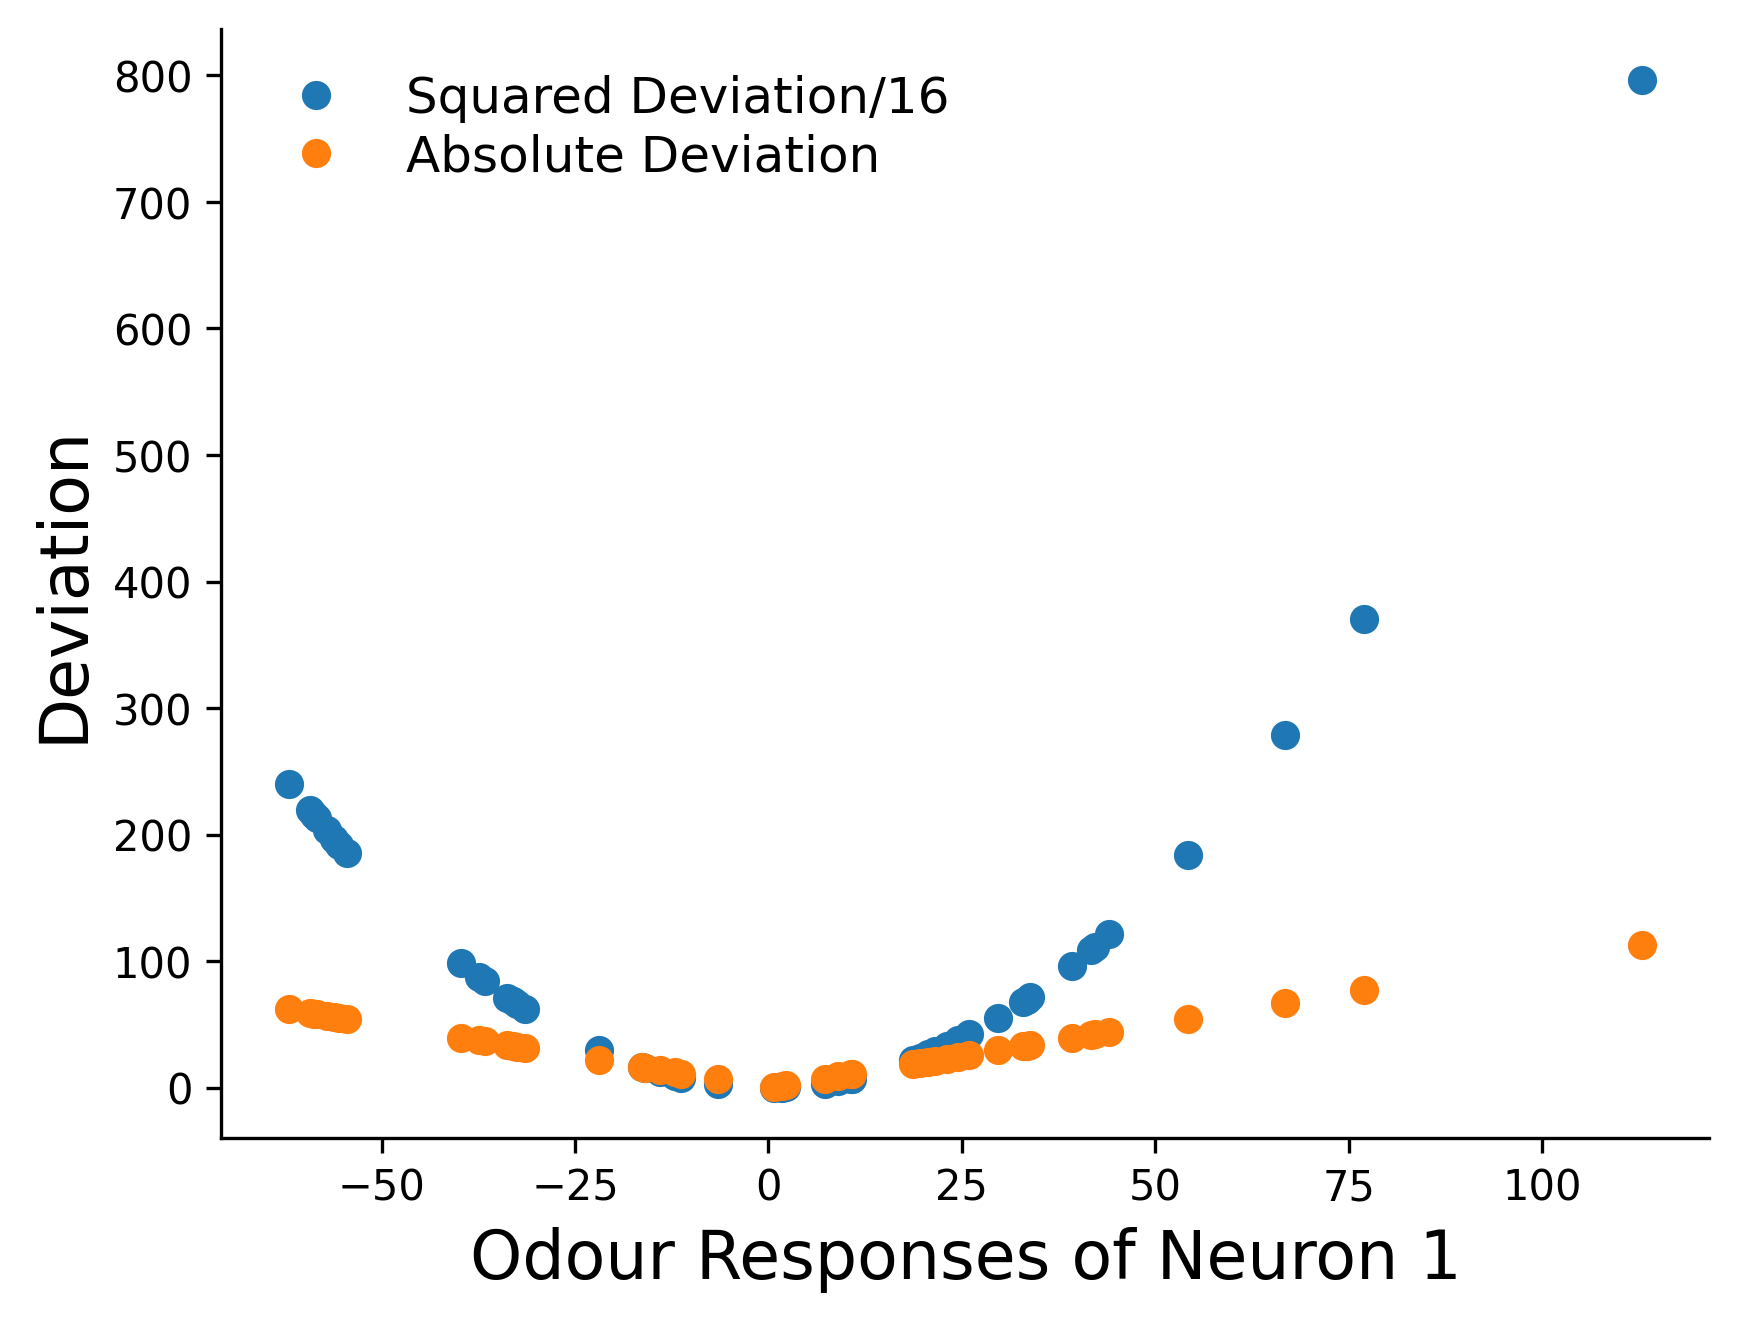
\includegraphics[width=0.5\textwidth]{figures/variance_vs_mad.png}
\end{center}
\end{frame}
\begin{frame}[label={sec:org78486a9}]{Covariance of neural populations}
\begin{itemize}
\item Neurons don't respond independently, but frequently \textbf{co}vary
\end{itemize}
\begin{center}
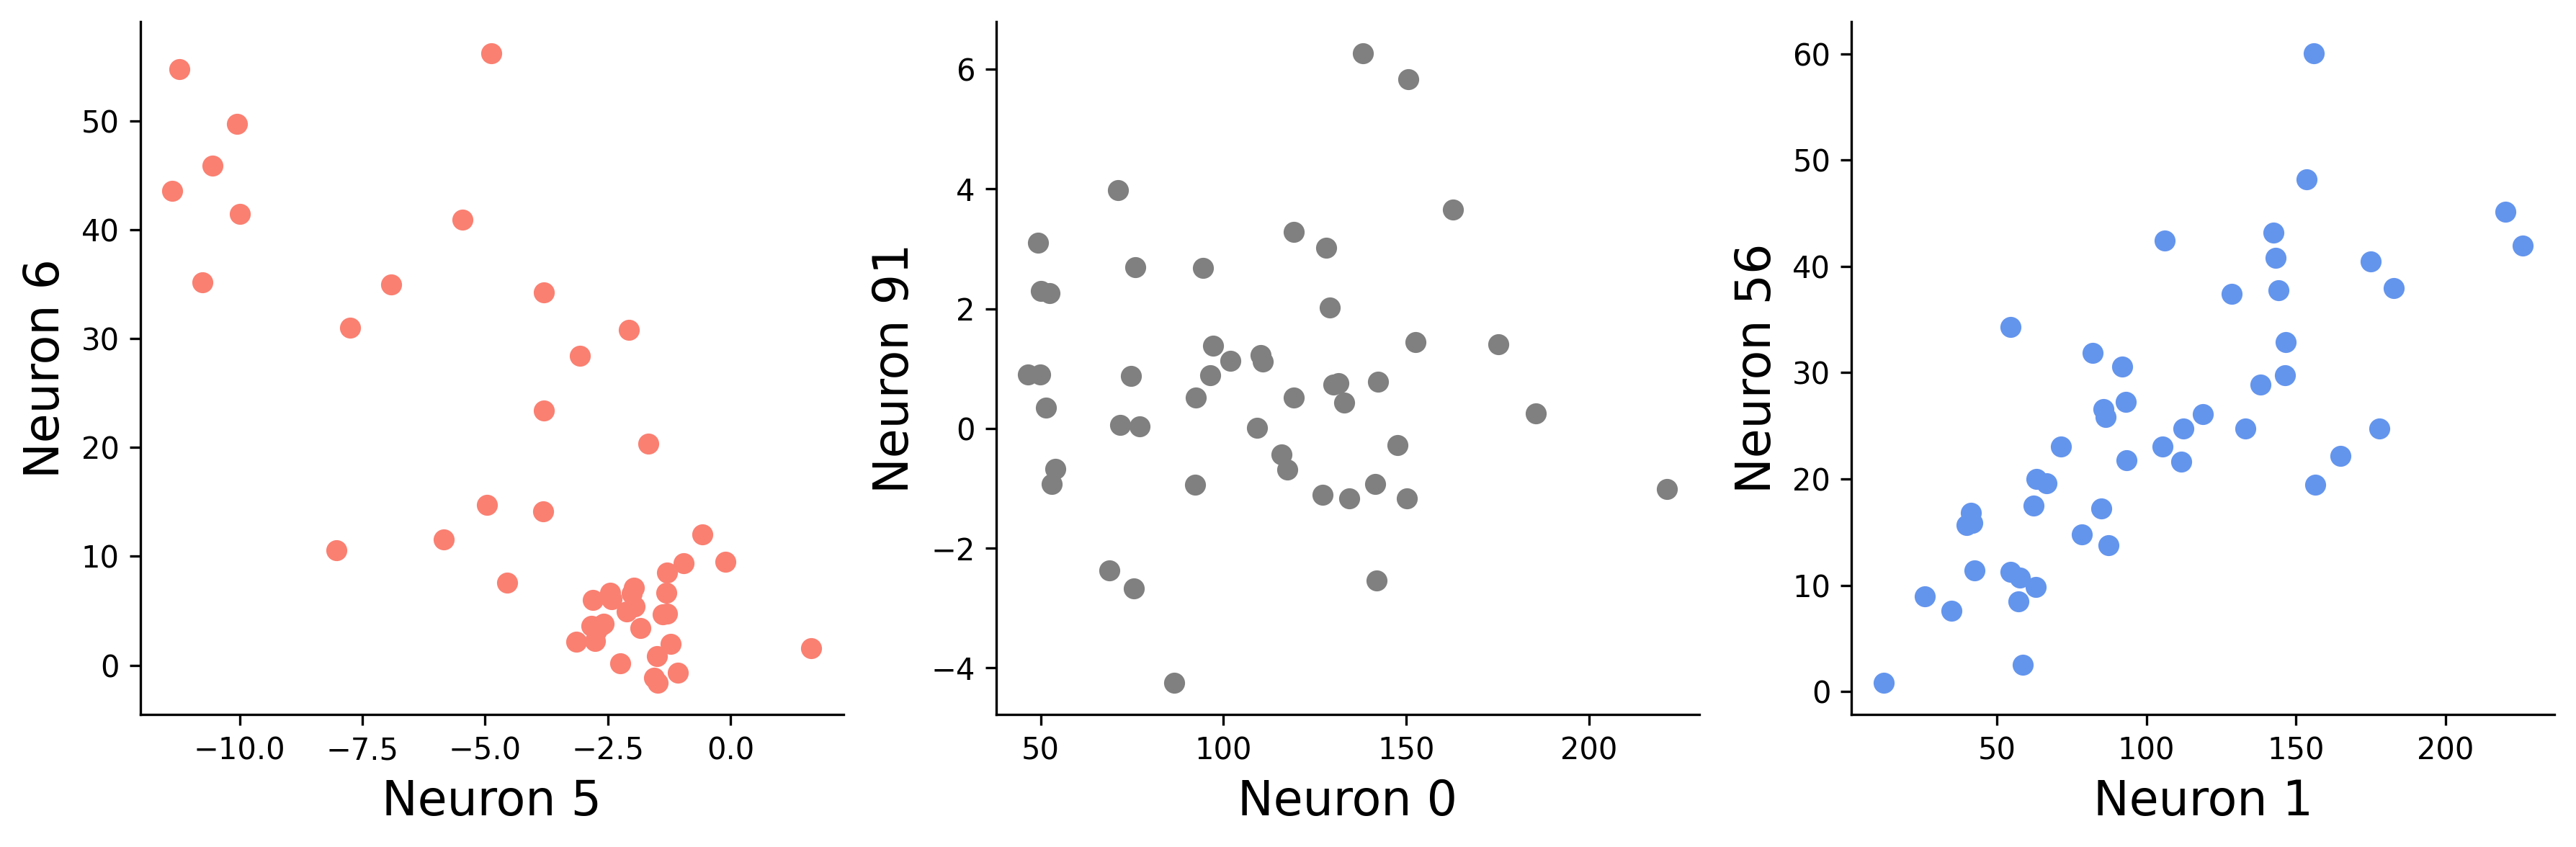
\includegraphics[width=1.0\textwidth]{figures/correlation.png}
\end{center}  
\begin{itemize}
\item \color{red}\textbf{Co}\color{black}variance measures covariation of a neuron with another:
$$ \cov(x_1, x_2) &= \langle (x_{1,\mu} - \overline{x}_1)(x_{\red{2},\mu} - \overline{x}_{\red{2}}) \rangle.$$
\item Variance is covariation of a neuron with itself!
\begin{align*} \var(x_1) &= \langle (x_{1,\mu} - \overline{x}_1)^2 \rangle\\
&= \langle (x_{1,\mu} - \overline{x}_1)(x_{1,\mu} - \overline{x}_1) \rangle.
\end{align*}
\end{itemize}
\end{frame}
\begin{frame}[label={sec:org0e1e6b6}]{Covariance matrix}
\begin{itemize}
\item The \textbf{covariance matrix} tabulates covariance for all pairs of neurons.
\[\cov(\xx) = \begin{bmatrix}\var(x_1) & \cov(x_1, x_2) & \dots \\ \cov(x_1, x_2) & \var(x_2) & \dots \\ \vdots & \vdots & \ddots \end{bmatrix} = \langle (\xx_\mu - \overline{\xx})(\xx_\mu - \overline{\xx})^T \rangle \]
\item Diagonals have variances
\item Off-diagonals have covariances
\end{itemize}
\begin{center}
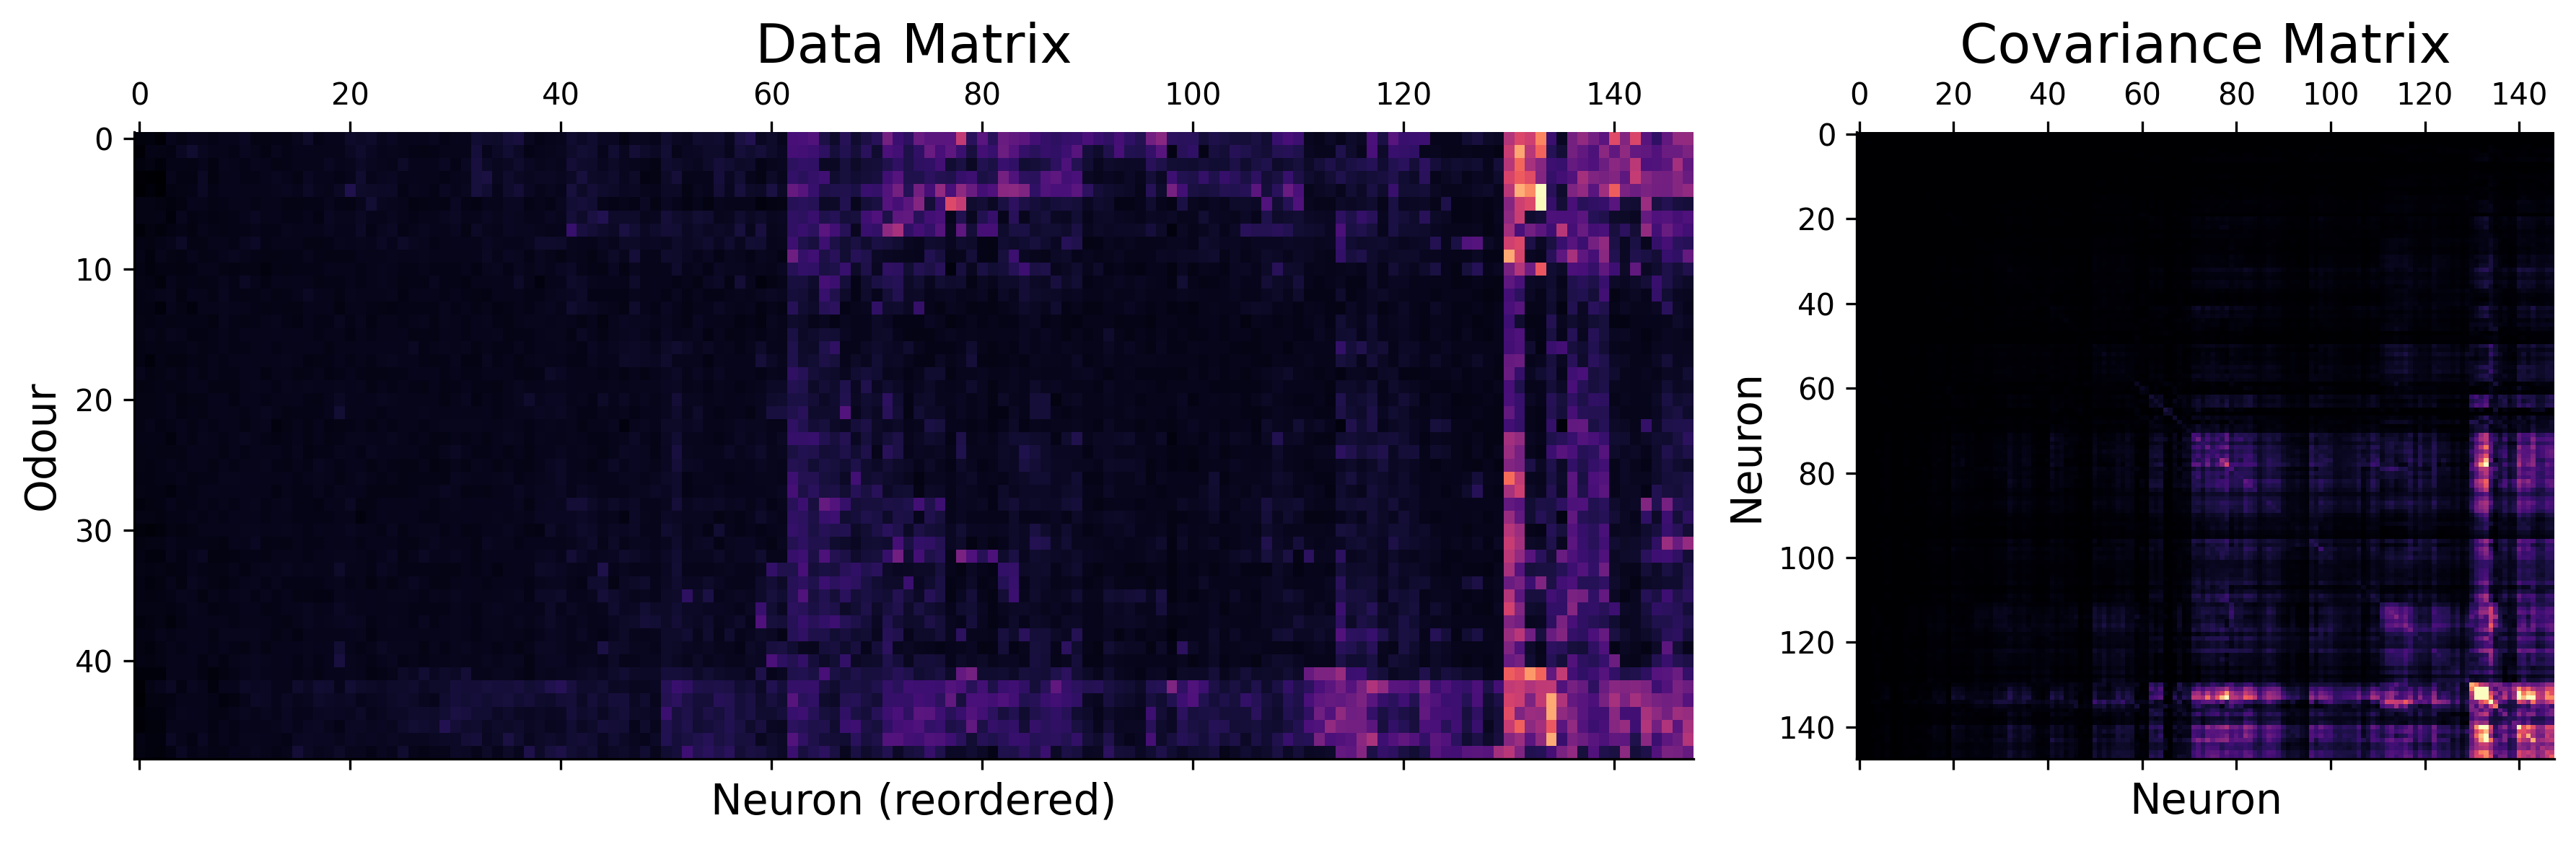
\includegraphics[width=1.0\textwidth]{figures/covariance_matrix.png}
\end{center}  
\begin{itemize}
\item Not just useful book keeping\ldots{}
\end{itemize}
\end{frame}
\section{Variance of Pseudo-Neurons}
\label{sec:org7e9a2a2}
\begin{frame}[label={sec:org27d4c14}]{Where we're going}
\begin{itemize}
\item Remember: PCA is about finding \bold{directions} that maximize variance:
\end{itemize}
\begin{center}
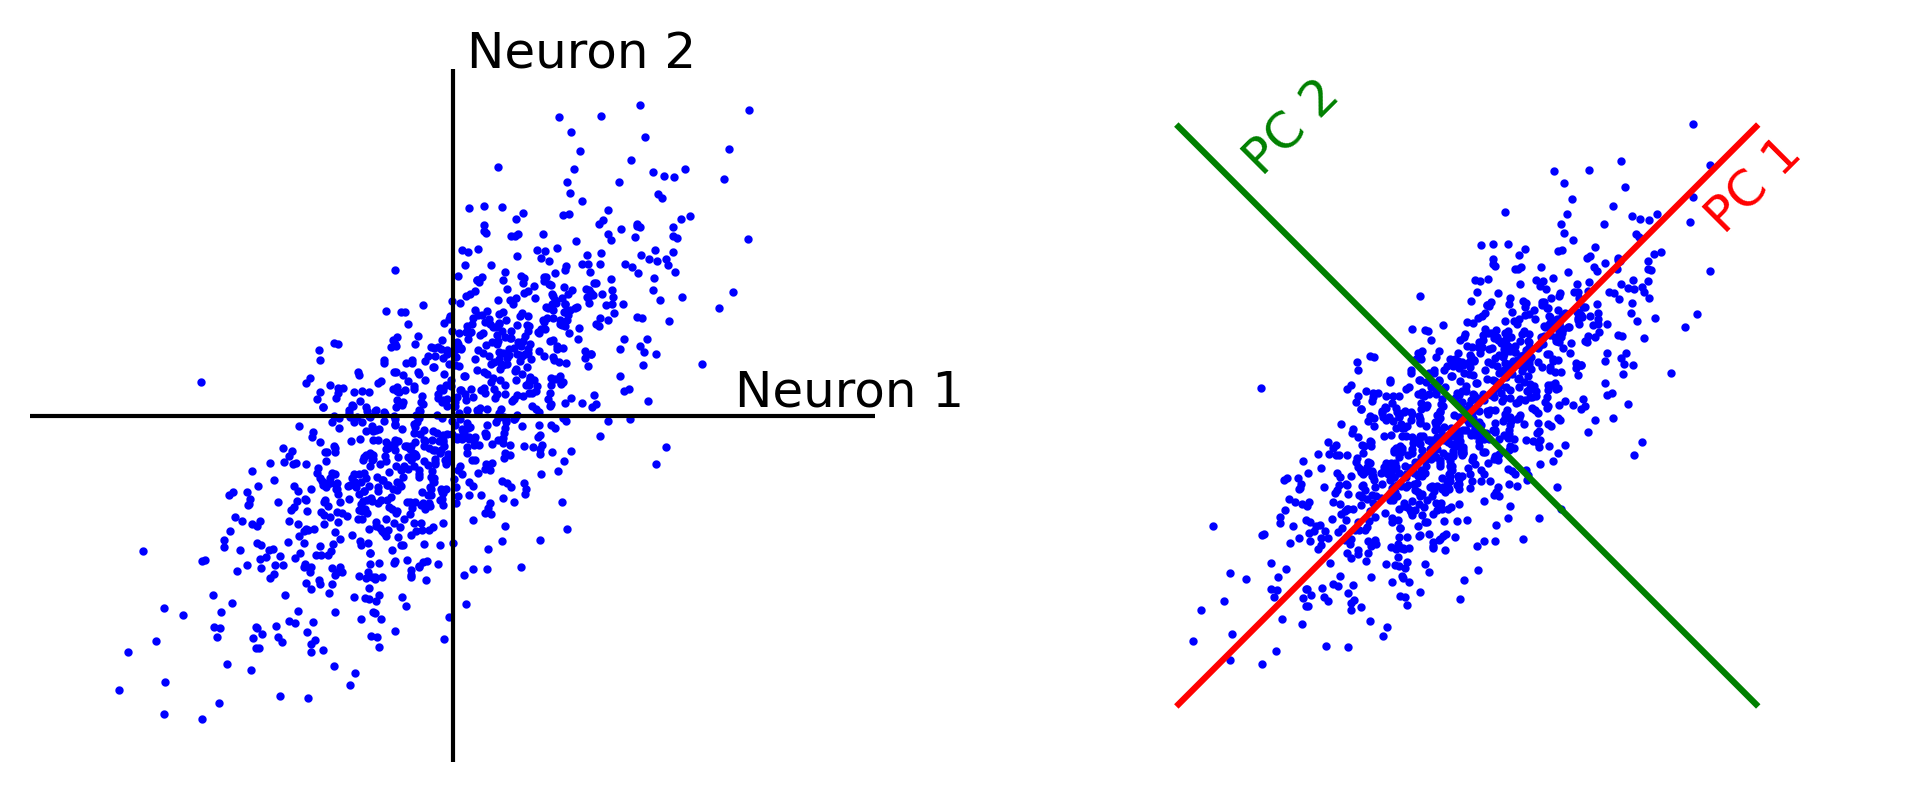
\includegraphics[width=1.0\textwidth]{figures/pca_illustration.png}
\end{center}
\begin{itemize}
\item The standard coordinate directions correspond to single neurons.
\item The variance of single neurons is variance along these directions.
\item We can define other directions as \bold{pseudo-neurons}.
\item The variance of pseudo-neurons is variance along these directions.
\item PCA = find the pseudo-neurons with the largest variance.
\end{itemize}
\end{frame}
\begin{frame}[label={sec:org4529351}]{Variance of a single neuron from covariance}
\begin{itemize}
\item Previously we just `took' the data \(x_{1,\mu}\)  for neuron 1.
\item This is projecting the population vector \(\xx_\mu\) along the first coordinate: $$x_{1,\mu} = \xx_\mu^T \ee_1.$$
\item We can then compute the mean activity
\begin{align*}
\overline{x}_1 &= \langle \xx_\mu^T \ee_1 \rangle = \langle \xx_\mu \rangle^T \ee_1 = \overline{\xx}^T  \ee_1.
\end{align*}
\item The variance is then
\end{itemize}
\begin{align*}
 \var(x_1) &= \langle (x_{1,\mu}- \overline{\tilde x}_1)^2 \rangle \\
&= \langle \left( \xx_\mu^T \ee_1  - \overline{\xx}_\mu^T \ee_1 \right)^2 \rangle\\
&= \langle \left( (\xx_\mu - \overline{\xx})^T\ee_1 \right)^2 \rangle\\
&= \langle \ee_1^T(\xx_\mu - \overline{\xx})  (\xx_\mu - \overline{\xx})^T\ee_1  \rangle\\
&= \ee_1^T \langle (\xx_\mu - \overline{\xx}) (\xx_\mu - \overline{\xx})^T \rangle \ee_1\\
&= \ee_1^T \cov(\xx) \ee_1.
\end{align*}
\begin{itemize}
\item So, the variance of neuron 1 is \bold{covariance along $\ee_1$}.
\end{itemize}
\end{frame}
\begin{frame}[label={sec:org4e2f92f}]{Other orthonormal coordinates define pseudo-neurons}
\begin{itemize}
\item Previously we described population activity in terms of standard coordinates \(\ee_1, \ee_2, \dots\) of neurons:
$$ \xx = x_1 \ee_1 + x_2 \ee_2 + \dots $$
\item We can describe the same activity \(\xx\) in other orthonormal coordinates \(\tilde \ee_1, \tilde \ee_2, \dots\) of \bold{pseudo-neurons}:
\end{itemize}
$$ \xx = \tilde x_1 \tilde \ee_1 + \tilde x_2 \tilde \ee_2 + \dots $$
\begin{figure}[htbp]
\centering
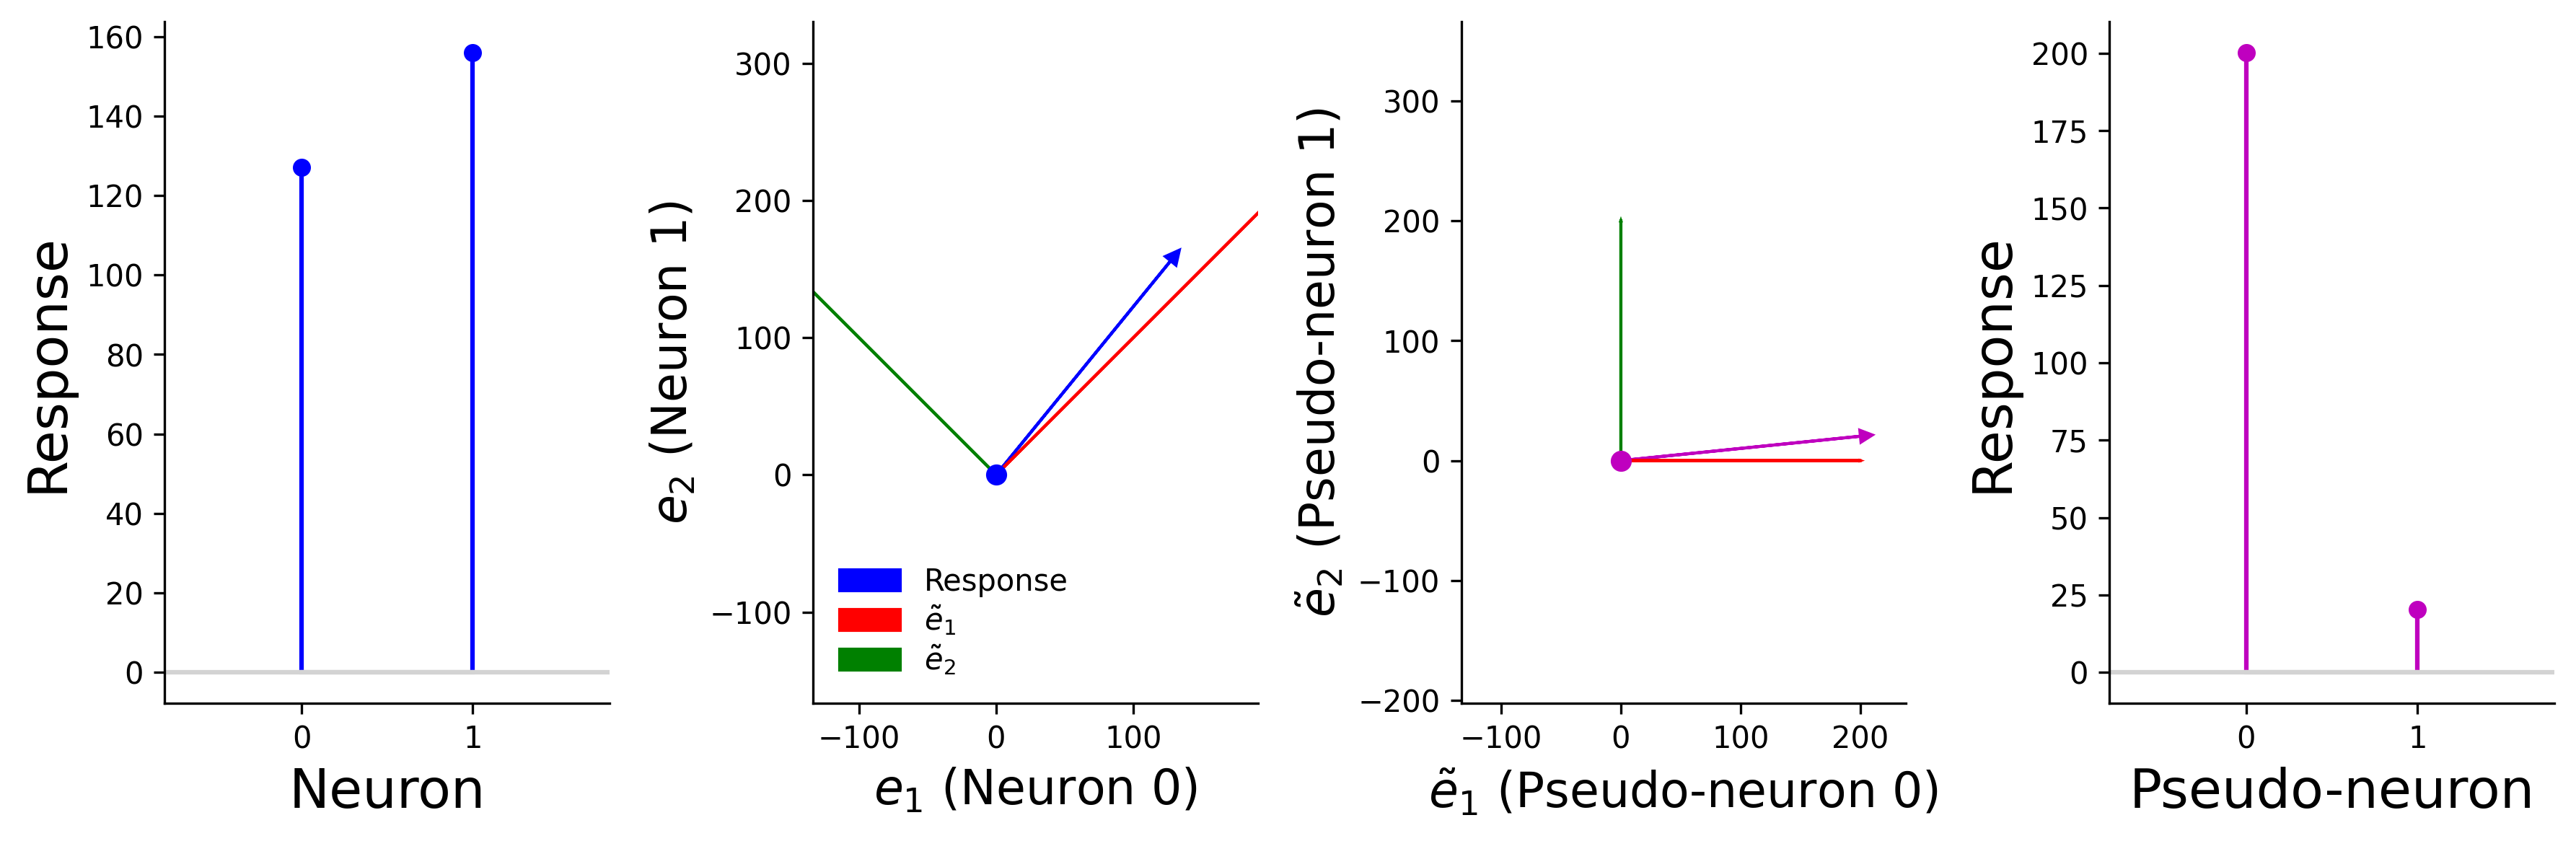
\includegraphics[width=1.0\textwidth]{figures/coordinate_transform.png}
\caption{Responses of neurons and pseudo-neurons to the first odour.}
\end{figure}
\end{frame}
\begin{frame}[label={sec:org5a30a20}]{Variance of a pseudo-neuron along \(\uu_1\)}
\begin{itemize}
\item Activity of the \bold{pseudo}neuron: $$\tilde x_{1,\mu} = \xx_\mu^T \uu_1.$$
\item Mean activity of the pseudoneuron:
\begin{align*}
\overline{\tilde x}_1 &= \langle \xx_\mu^T \uu_1 \rangle = \langle \xx_\mu \rangle^T \uu_1 = \overline{\xx}^T  \uu_1.
\end{align*}
\item The variance is then
\end{itemize}
\begin{align*}
 \var(\tilde x_1) &= \langle (\tilde x_{1,\mu}- \overline{\tilde x}_1)^2 \rangle \\
&= \langle \left( \xx_\mu^T \uu_1  - \overline{\xx}_\mu^T \uu_1 \right)^2 \rangle\\
&= \langle \left( (\xx_\mu - \overline{\xx})^T\uu_1 \right)^2 \rangle\\
&= \langle \uu_1^T(\xx_\mu - \overline{\xx})  (\xx_\mu - \overline{\xx})^T\uu_1  \rangle\\
&= \uu_1^T \langle (\xx_\mu - \overline{\xx}) (\xx_\mu - \overline{\xx})^T \rangle \uu_1\\
&= \uu_1^T \cov(\xx) \uu_1.
\end{align*}
\begin{itemize}
\item So, the variance of the pseudoneuron is \bold{covariance along $\uu_1$}.
\end{itemize}
\end{frame}
\begin{frame}[label={sec:org1ee8960}]{Variance of \emph{any} pseudoneuron}
\begin{itemize}
\item Following the pattern, variance of a pseudoneuron \(\tilde x = \xx^T\uu\) is 
$$ \var(\tilde x) = \uu^T \cov(\xx) \uu.$$
\item PCA now becomes finding the \(\uu\) that maximizes this variance.
\item How do we do this? By decomposing the covariance matrix!
\item But first\ldots{}
\end{itemize}
\end{frame}
\section{Some Facts about Matrices}
\label{sec:orgb232b27}
\begin{frame}[label={sec:org76b084b}]{Matrices}
\begin{itemize}
\item Some matrices we've already encountered:
\end{itemize}
\begin{center}
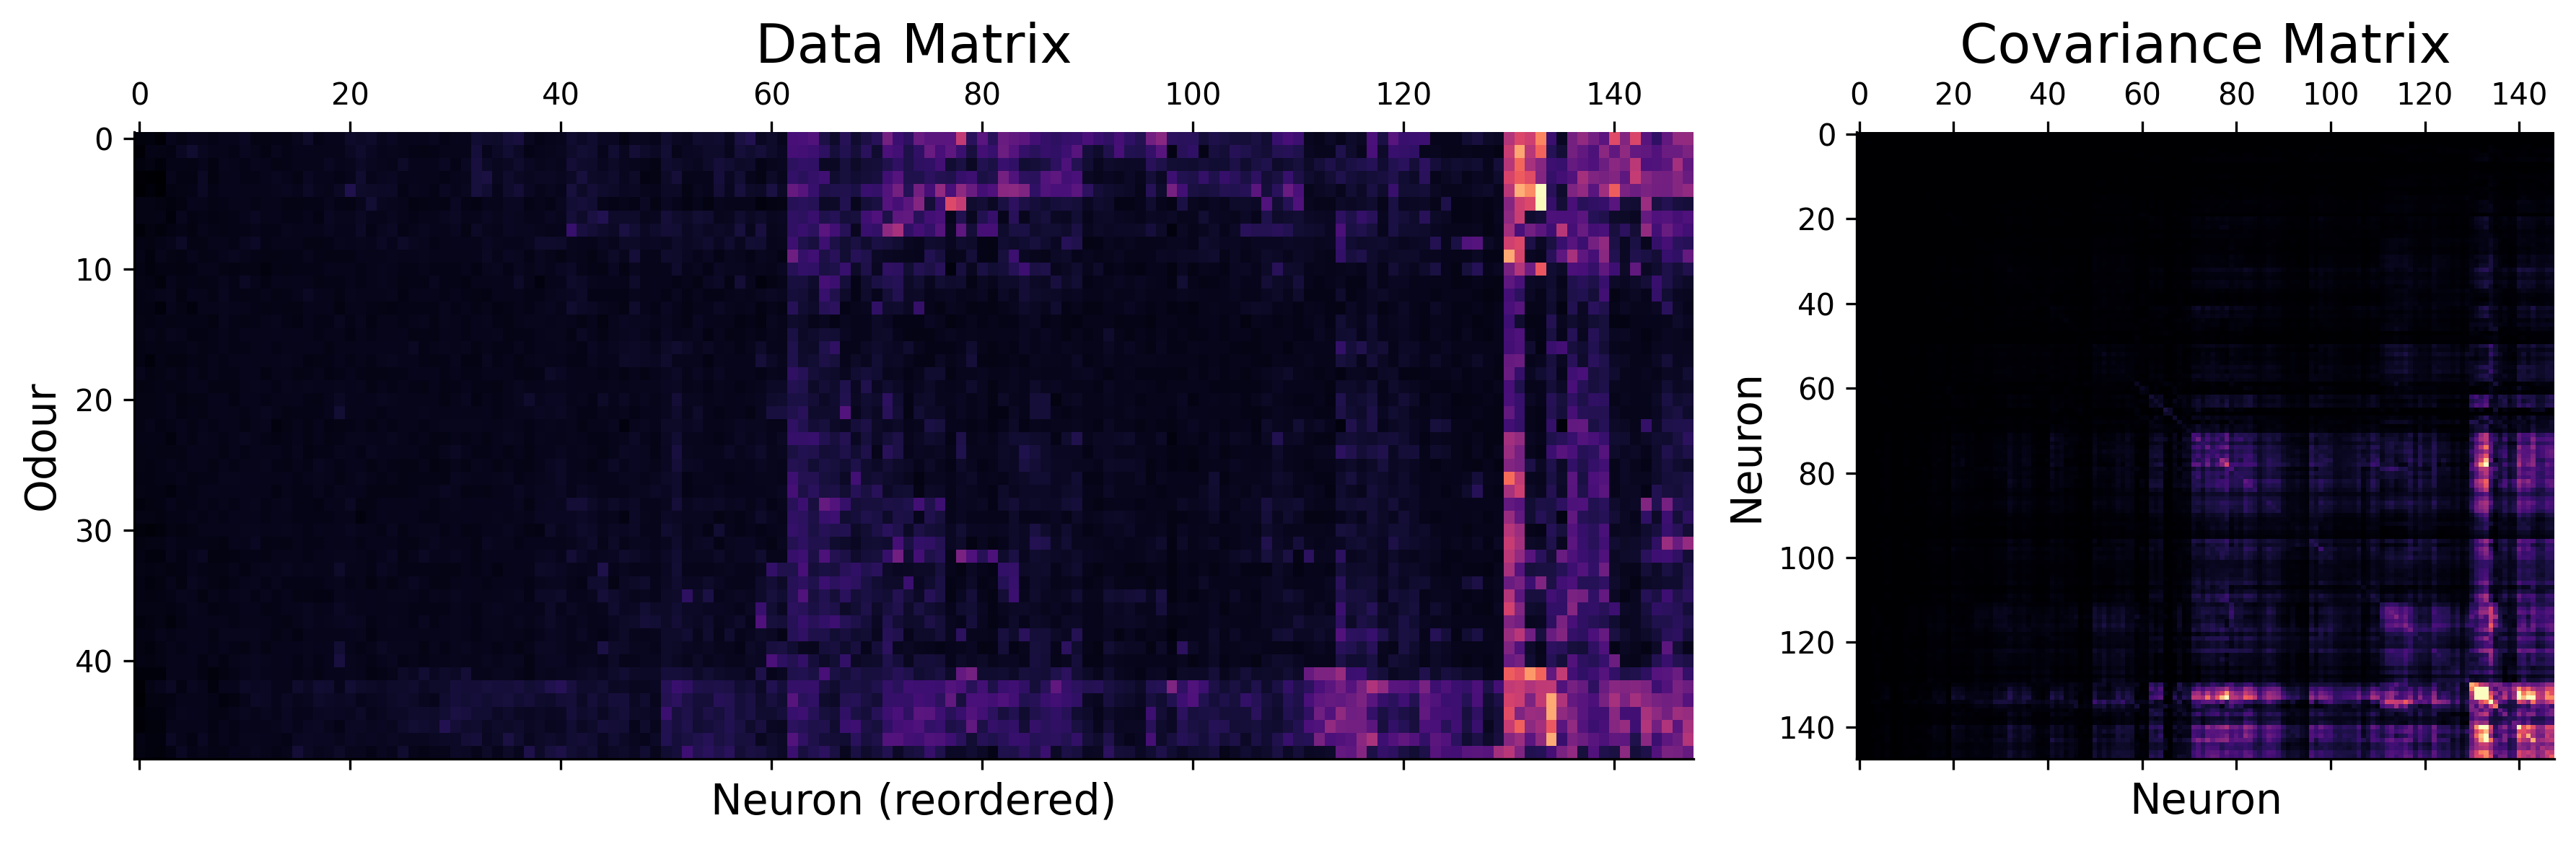
\includegraphics[width=1.0\textwidth]{figures/covariance_matrix.png}
\end{center}  
\begin{itemize}
\item Data matrix (rectangular)
\item Covariance matrix (square, symmetric)
\begin{itemize}
\item Why is it symmetric?
\end{itemize}
\end{itemize}
\end{frame}
\begin{frame}[label={sec:org9b5ddea}]{Different ways to view matrices}
\[ \mathbf{A} = \underbrace{\begin{bmatrix} A_{11}, & A_{12}, & \dots \\ A_{21}, & A_{22} & \dots \\ \vdots & \vdots & \ddots \end{bmatrix}}_{\text{Table of elements}} = \underbrace{\begin{bmatrix} \rr_1^T \\ \rr_2^T \\ \vdots \\ \rr_M^T \end{bmatrix}}_{\text{Stacked rows}} = \underbrace{\begin{bmatrix} \cc_1,& \cc_2, & \cc_3, & \dots & \cc_N \end{bmatrix}}_{\text{Stacked columns}}. \]
\end{frame}
\begin{frame}[label={sec:orgb58b725}]{Matrix operations}
\begin{itemize}
\item \bold{Linearly} transform N-dimensional inputs \(\xx\) into M-dimensional outputs \(\yy\), \[ \yy = \mathbf{A} \xx.\]
\item Can think of this element-wise:
$$ y_i = \sum_{j=1}^N A_{ij} x_j.$$
\item Can think of this as projecting \(\xx\) on each row,
$$ \yy = \begin{bmatrix} y_1 \\ y_2\\ \vdots\\ y_M \end{bmatrix} = \begin{bmatrix} \rr_1^T \xx \\ \rr_2^T \xx \\ \vdots\\ \rr_M^T \xx \end{bmatrix}.$$
\item Can think of this as summing the columns, weighted by \(\xx\),
$$ \yy = \sum_{i=1}^N \cc_i x_i.$$
\end{itemize}
\end{frame}
\begin{frame}[label={sec:org427465c}]{Example Matrices}
\centering
\begin{array}{l c l}
\textbf{Name} & \textbf{Matrix } \mathbf{A}  & \textbf{Action } \yy = \mathbf{A} \xx \\ \hline
\text{Zero} & \begin{bmatrix} 0 & 0 \\ 0 & 0 \end{bmatrix} & \yy = \mathbf{0} \\[10pt]
\text{Identity} & \begin{bmatrix} 1 & 0 \\ 0 & 1 \end{bmatrix} & \yy = \xx \\[10pt]
\text{All ones} & \begin{bmatrix} 1 & 1 \\ 1 & 1 \end{bmatrix} & \yy = \begin{bmatrix}\sum_i x_i \\ \sum_i x_i \end{bmatrix} \\[10pt]
\text{Uniform scaling} & \begin{bmatrix} k & 0 \\ 0 & k \end{bmatrix} & \yy = \begin{bmatrix} k  x_1  \\ k x_2 \end{bmatrix} \\[10pt]
\text{Diagonal} & \begin{bmatrix} a & 0 \\ 0 & b \end{bmatrix} & \yy = \begin{bmatrix} a x_1 \\ b x_2 \end{bmatrix} \\[10pt]
\text{Permutation} & \begin{bmatrix} 0 & 1 \\ 1 & 0 \end{bmatrix} & \yy = \begin{bmatrix} x_2 \\ x_1 \end{bmatrix} \\[10pt]
\text{Rotation} & \begin{bmatrix} \cos \theta & -\sin \theta \\ \sin \theta & \cos \theta \end{bmatrix} & \yy \text{ is $\xx$ rotated by $\theta$.}
\end{array}
\end{frame}
\begin{frame}[label={sec:orgef95a68}]{Composing transformations}
\begin{itemize}
\item We can form complex transformations by composing simple ones.
\item For example, a scaling and a rotation:
\end{itemize}
$$ \yy = \underbrace{\begin{bmatrix} a & 0 \\ 0 & b \end{bmatrix}}_{\text{scaling}} \underbrace{\begin{bmatrix} \cos \theta & -\sin \theta \\ \sin \theta & \cos \theta \end{bmatrix}}_{\text{rotation}} \begin{bmatrix} x_1 \\ x_2 \end{bmatrix} = \underbrace{\mathbf{D R}}_{\mathbf A} \xx.$$
\end{frame}
\section{Singular Value Decomposition}
\label{sec:orgf2eb6dd}
\begin{frame}[label={sec:org2ec7e0a}]{All matrices are diagonal matrices (in the right coordinates)}
\begin{itemize}
\item Diagonal matrices were easy to work with
\end{itemize}
\begin{center}
\begin{bmatrix} a & 0 \\ 0 & b \end{bmatrix} \begin{bmatrix} x_1 \\ x_2 \end{bmatrix} = \begin{bmatrix} a x_1 \\ b x_2 \end{bmatrix}
\end{center}
\begin{itemize}
\item What about an arbitrary matrix? Looks complex\ldots{}
\end{itemize}
\begin{center}
\begin{bmatrix} A_{11} & A_{12} \\ A_{21} & A_{22} \end{bmatrix} \begin{bmatrix} x_1 \\ x_2 \end{bmatrix} = \begin{bmatrix}  \sum_j A_{1j} x_j \\ \sum_j A_{2j} x_j \end{bmatrix}.
\end{center}
\begin{itemize}
\item Surprise: Every matrix \(\AA\) is the composition of just three operations!
$$ \AA  = \underbrace{\UU}_{\text{rotate}} \underbrace{\SS}_{\text{scale}} \underbrace{\VV^T}_{\text{project}}.$$
\end{itemize}
\end{frame}
\begin{frame}[label={sec:org8cac9d2}]{Three parts of Singular Value Decomposition}
$$ \AA  = \underbrace{\UU}_{\text{rotate}} \underbrace{\SS}_{\text{scale}} \underbrace{\VV^T}_{\text{project}}.$$
\begin{itemize}
\item Columns of \(\VV\) form orthonormal coordinates for the \bold{input} space.
\item Columns of \(\UU\) form orthonormal coordinates for the \bold{output} space
\item Diagonal matrix \(\SS\) of non-negative \bold{singular values} apply a scaling.
\item If we:
\begin{itemize}
\item Use \(\VV\) coordinates for the input, and
\item Use \(\UU\) coordinates for the output, then
\item \(\AA\) is a scaling!
\end{itemize}
\end{itemize}
\end{frame}
\begin{frame}[label={sec:org4748740}]{Three transformations in Singular Value Decomposition}
\begin{figure}[htbp]
\centering
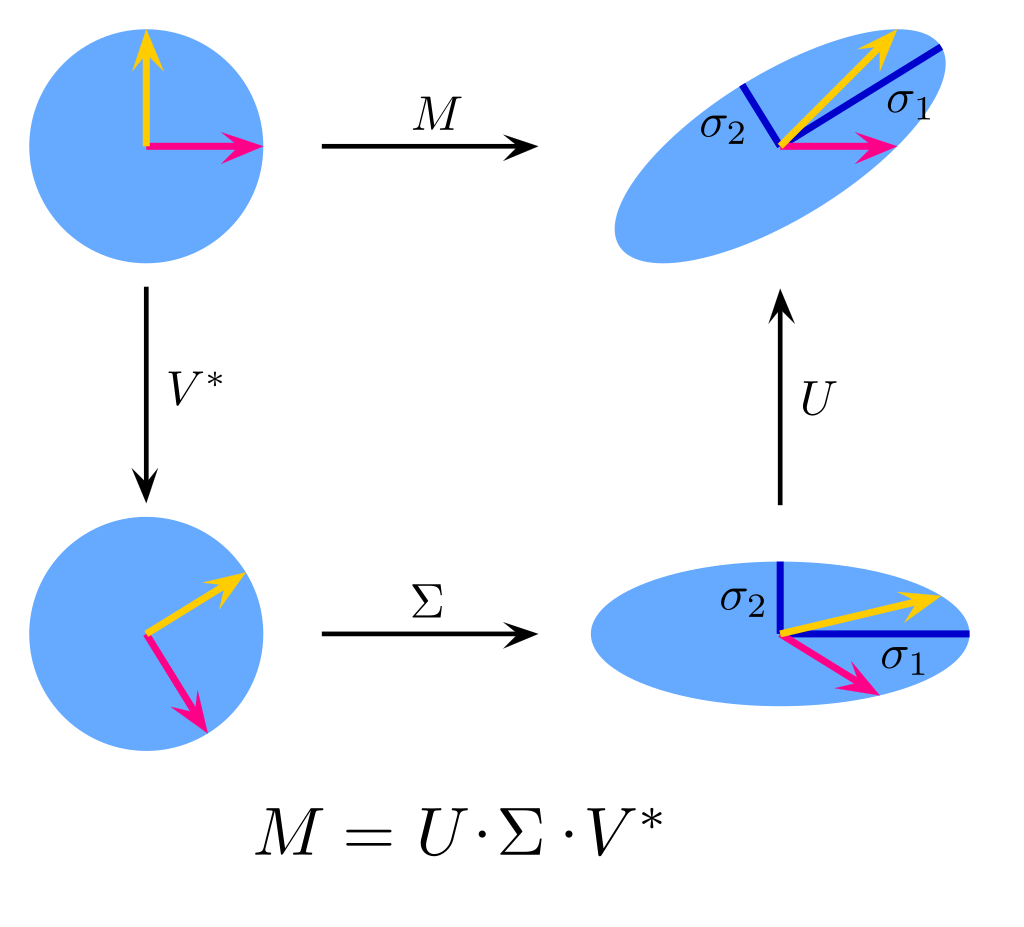
\includegraphics[width=0.6\textwidth]{figures/svd_parts.png}
\caption{Three transformations in Singular Value Decomposition (Wikipedia).}
\end{figure}  
\end{frame}
\begin{frame}[label={sec:org0be965e}]{Three matrices of Singular Value Decomposition}
\begin{figure}[htbp]
\centering
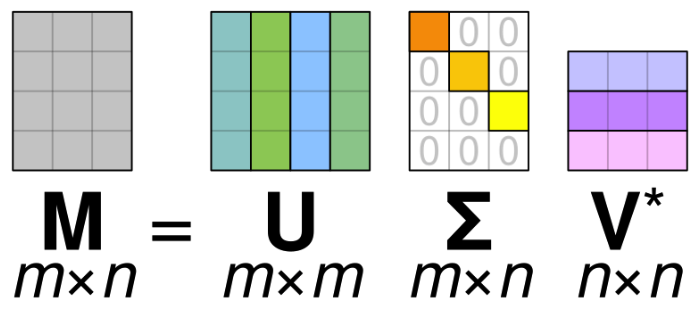
\includegraphics[width=0.8\textwidth]{figures/svd_blocks.png}
\caption{Three matrices of Singular Value Decomposition (Wikipedia).}
\end{figure}
\end{frame}
\begin{frame}[label={sec:orgbd1f0dd}]{Three steps of Singular Value Decomposition}
$$ \AA \xx = \underbrace{\UU}_{\text{rotate}} \underbrace{\SS}_{\text{scale}} \underbrace{\VV^T}_{\text{project}} \xx.$$
\begin{enumerate}
\item Project \(\xx\) onto the input coordinates:
\[ \VV^T \xx = \begin{bmatrix} \vv_1^T \xx \\ \dots \\ \vv_N^T \xx \end{bmatrix} = \begin{bmatrix} \tilde x_1 \\ \dots \\ \tilde x_N \end{bmatrix} \]
\item Scale by \(\SS\):
\[ \SS \VV^T \xx = \begin{bmatrix} s_1 & 0 & \dots \\ 0 & s_2 & \dots \\ \vdots & \vdots & \ddots \\ \end{bmatrix} \begin{bmatrix} \tilde x_1 \\ \dots \\ \tilde x_N \end{bmatrix} = \begin{bmatrix} s_1 \tilde x_1 \\ s_2 \tilde x_2 \\ \dots \\ s_N \tilde x_N \end{bmatrix} \]
\item Project out using the output coordinates
\[ \UU \SS \VV^T \xx = [\uu_1, \uu_2, \dots, \uu_N] \begin{bmatrix}s_1 \tilde x_1 \\ s_2 \tilde x_2 \\ \dots \\ s_N \tilde x_N \end{bmatrix} = \uu_1 s_1 \tilde x_1 + \uu_2 s_2 \tilde x_2 + \dots  \]
\end{enumerate}
\end{frame}
\begin{frame}[label={sec:org3ec8748}]{SVD of simple matrices}
\centering
\begin{array}{l c c c c}
\textbf{Name} & \mathbf{A}  & \UU & \mathbf{s} & \VV \\ \hline
\text{Zero} & \begin{bmatrix} 0 & 0 \\ 0 & 0 \end{bmatrix} & \begin{bmatrix} 1 & 0 \\ 0 & 1 \end{bmatrix} & \begin{bmatrix} 0, & 0\end{bmatrix} & \begin{bmatrix} 1 & 0 \\ 0 & 1 \end{bmatrix} \\[10pt]
\text{Identity} & \begin{bmatrix} 1 & 0 \\ 0 & 1 \end{bmatrix} & \begin{bmatrix} 1 & 0 \\ 0 & 1 \end{bmatrix} & \begin{bmatrix} 1, & 1\end{bmatrix} & \begin{bmatrix} 1 & 0 \\ 0 & 1 \end{bmatrix} \\[10pt]
\text{Negation} & \begin{bmatrix} -1 & 0 \\ 0 & -1 \end{bmatrix} & \begin{bmatrix} -1 & 0 \\ 0 & -1 \end{bmatrix} & \begin{bmatrix} 1, & 1\end{bmatrix} & \begin{bmatrix} 1 & 0 \\ 0 & 1 \end{bmatrix} \\[10pt]
\text{All ones} & \begin{bmatrix} 1 & 1 \\ 1 & 1 \end{bmatrix} & {1\over \sqrt{2}}\begin{bmatrix} 1 & -1 \\ 1 & 1 \end{bmatrix} & \begin{bmatrix} 2, & 0\end{bmatrix} & {1 \over \sqrt{2}}\begin{bmatrix} 1 & 1 \\ -1 & 1 \end{bmatrix} \\[10pt]
\text{Diagonal} & \begin{bmatrix} 2 & 0 \\ 0 & 3 \end{bmatrix} & \begin{bmatrix} 1 & 0 \\ 0 & 1 \end{bmatrix} & \begin{bmatrix} 2, & 3\end{bmatrix} & \begin{bmatrix} 1 & 0 \\ 0 & 1 \end{bmatrix} \\[10pt]
\text{Permutation} & \begin{bmatrix} 0 & 1 \\ 1 & 0 \end{bmatrix} & \begin{bmatrix} 0 & 1 \\ 1 & 0 \end{bmatrix} & \begin{bmatrix} 1, & 1\end{bmatrix} & \begin{bmatrix} 0 & 1 \\ 1 & 0 \end{bmatrix} \\[10pt]
\text{Rotation by $\theta$} & \begin{bmatrix} \cos \theta & -\sin \theta \\ \sin \theta & \cos \theta \end{bmatrix} & \begin{bmatrix} \cos \theta & -\sin \theta \\ \sin \theta & \cos \theta \end{bmatrix} & \begin{bmatrix} 1, & 1\end{bmatrix} & \begin{bmatrix} 1 & 0 \\ 0 & 1 \end{bmatrix} \\[10pt] 
\end{array}
\end{frame}

\begin{frame}[label={sec:org9e8b6a9}]{SVD of covariance matrices}
\begin{itemize}
\item Remember why we care: we're after the variance of pseudoneurons $$\uu^T \cov(\xx) \uu.$$
\item For covariance matrices, the input and output coordinates are the same $$ \cov(\xx) = \VV \SS \VV^T $$
\item Equalizer: Inputs are analyzed in \(\VV\) coordinates and scaled. $$  \cov(\xx) \uu = \sum_i \vv_i \underbrace{s_i}_{\text{scale}} \underbrace{\vv_i^T \uu}_{\text{project}} $$
\end{itemize}
\end{frame}
\begin{frame}[label={sec:org65a601c}]{SVD and eigendecomposition}
\begin{itemize}
\item All matrices have SVDs: \(\mathbf{X} = \UU \SS \VV^T\)
\item For covariance matrices, the input and output coordinates are the same: \(\cov(\xx) \propto \VV \SS^2 \VV^T\)
\item Also known as the \bold{eigendecomposition} of the covariance matrix.
\item The right singular vectors \(\VV\) of the data matrix are the eigenvectors/singular vectors of the covariance matrix.
\item The singular values of the data matrix and the cov. matrix are closely related:
\begin{align*}
\text{Singular values of cov. matrix} &= \text{Eigenvalues of the cov. matrix}\\
 &\propto \text{\bold{Squared} sing. values of the data matrix.}
 \end{align*}
\end{itemize}
\end{frame}

\begin{frame}[label={sec:org9f2bf32}]{Maximum variance direction from SVD}
\begin{itemize}
\item We can use SVD to read-off the maximum variance direction(s) we need!
\item Variance along a direction \(\uu\)
\begin{align*} \uu^T \cov(\xx) \uu &= \uu^T \underbrace{\left(\sum_i \vv_i s_i \vv_i^T\right)}_{\text{SVD}} \uu\\
&= \sum_i (\uu^T \vv_i) s_i (\vv_i^T \uu)\\
&= \sum_i s_i (\vv_i^T \uu)^2
\end{align*}
\item Maximum variance direction is \(\vv_1\)
\item Next highest variance direction is \(\vv_2\), etc.
\end{itemize}
\end{frame}
\section{Dimensionality Reduction with PCA}
\label{sec:org5bcf51b}
\begin{frame}[label={sec:org6a62deb}]{Finally: Dimension Reduction with PCA}
\begin{itemize}
\item Project data onto maximum variance directions: \(\widetilde{\mathbf{X}} = \mathbf{X} \VV.\)
\end{itemize}
\begin{center}
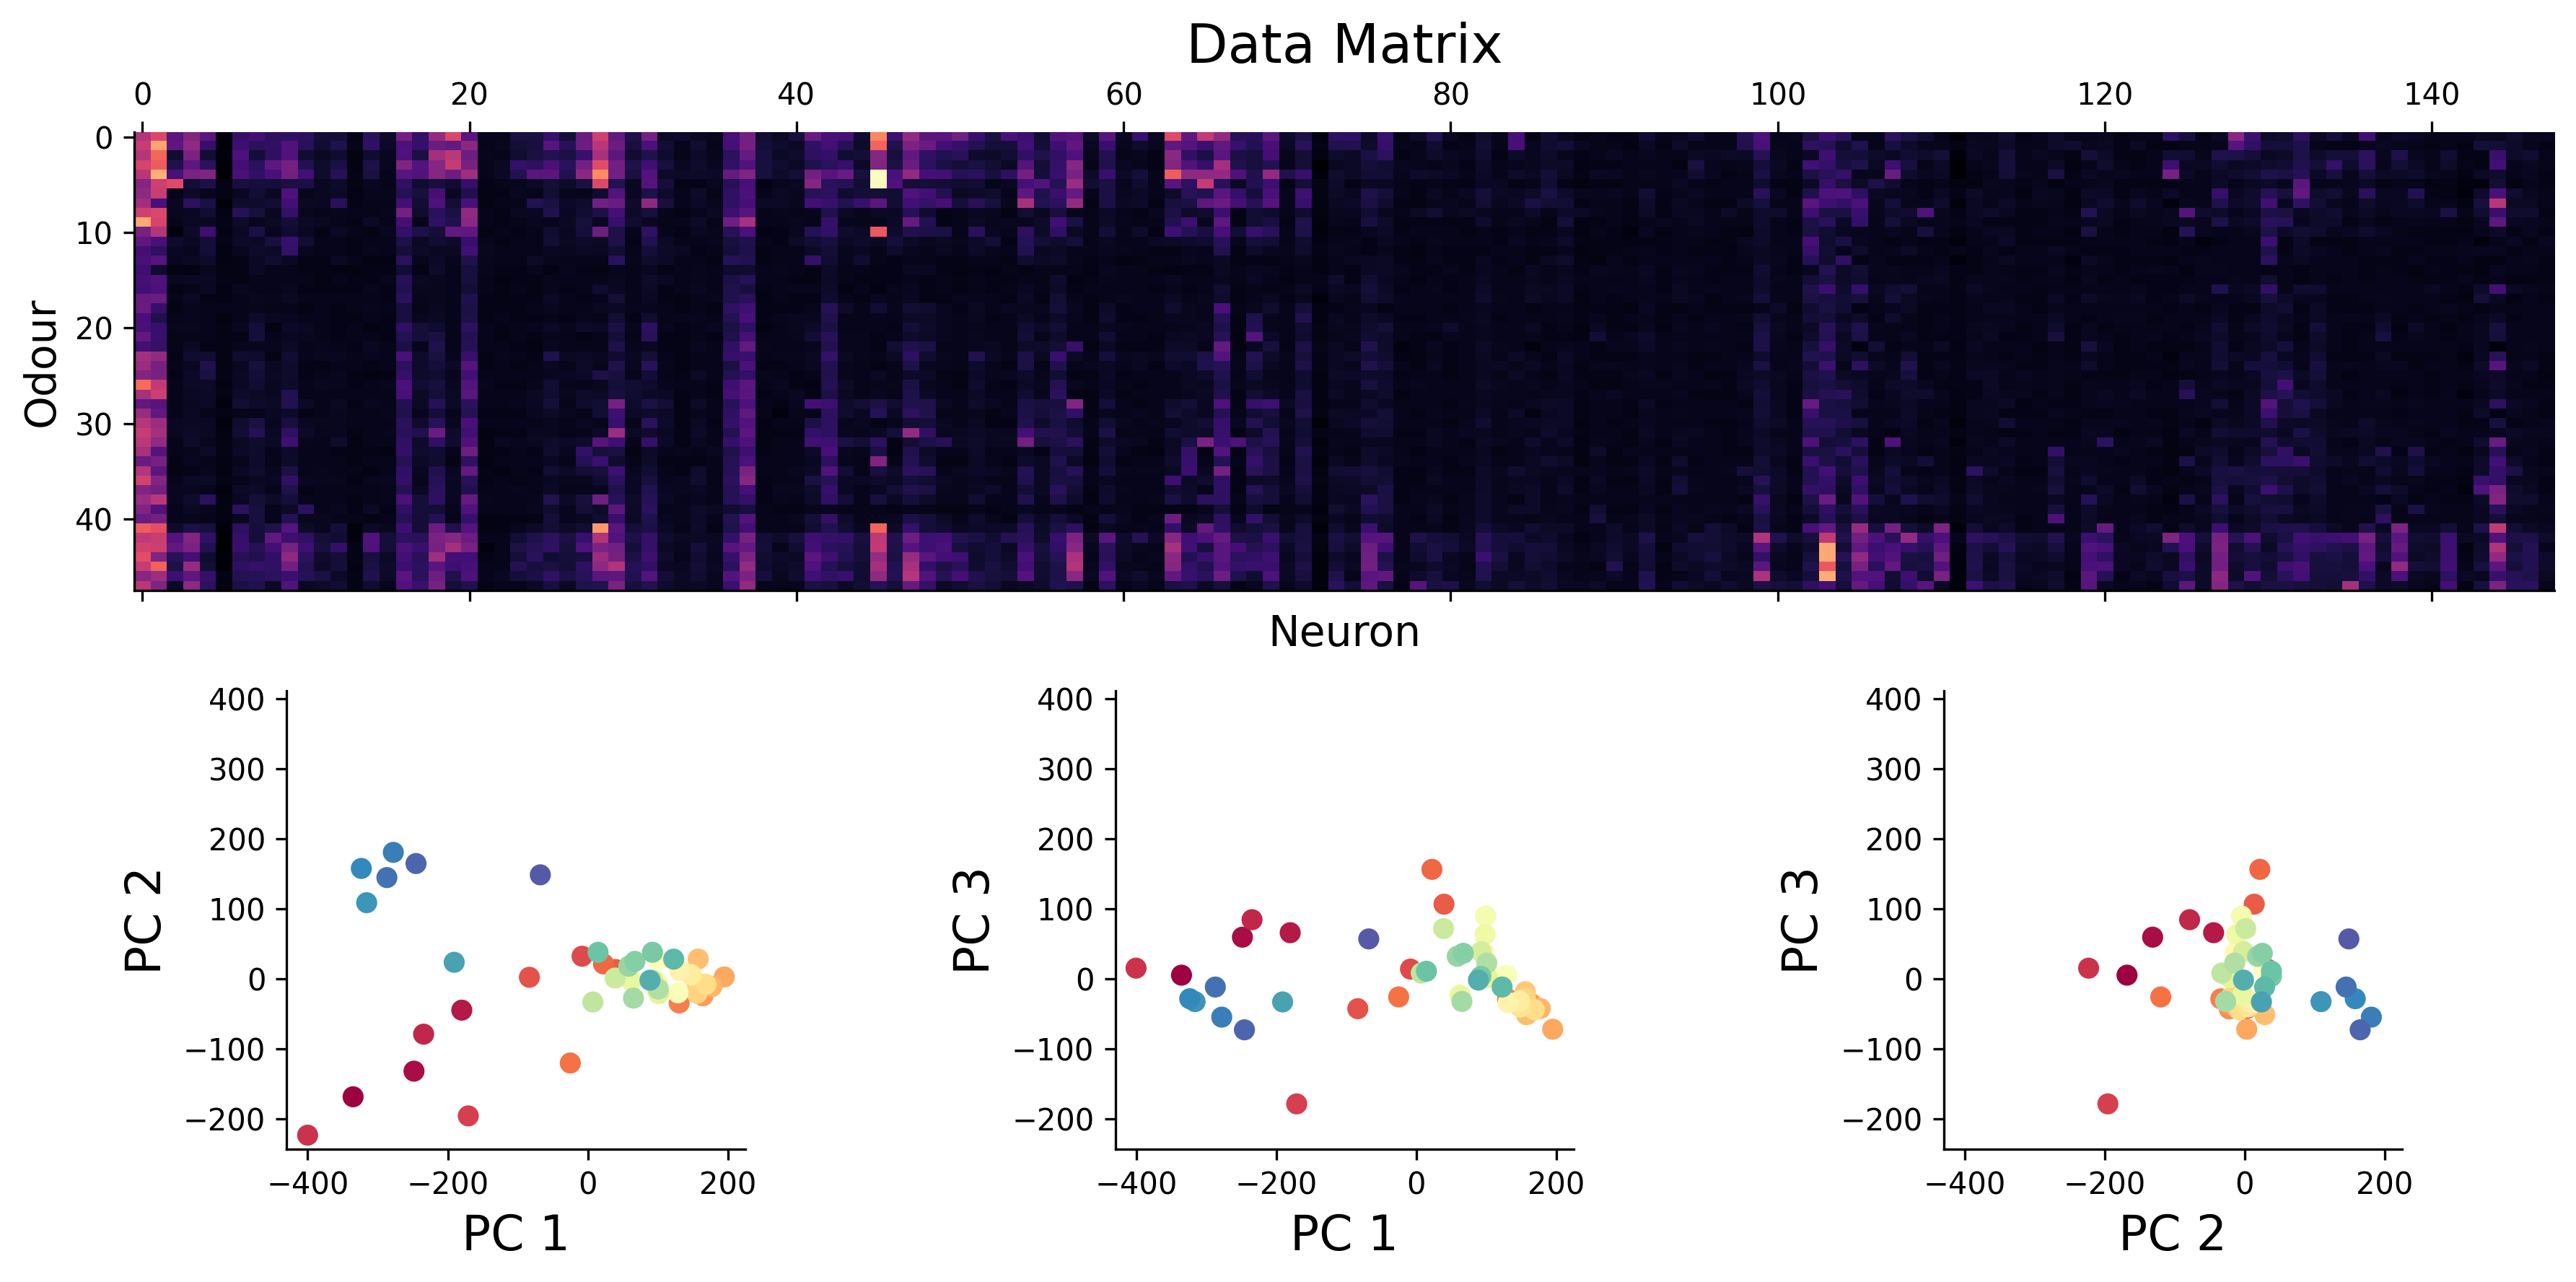
\includegraphics[width=1.0\textwidth]{figures/pca_projections.png}
\end{center}
\begin{itemize}
\item Notice: projections are decorrelated
\end{itemize}
\end{frame}
\begin{frame}[label={sec:org1dd0bc3}]{Examining the Principal Components}
\begin{center}
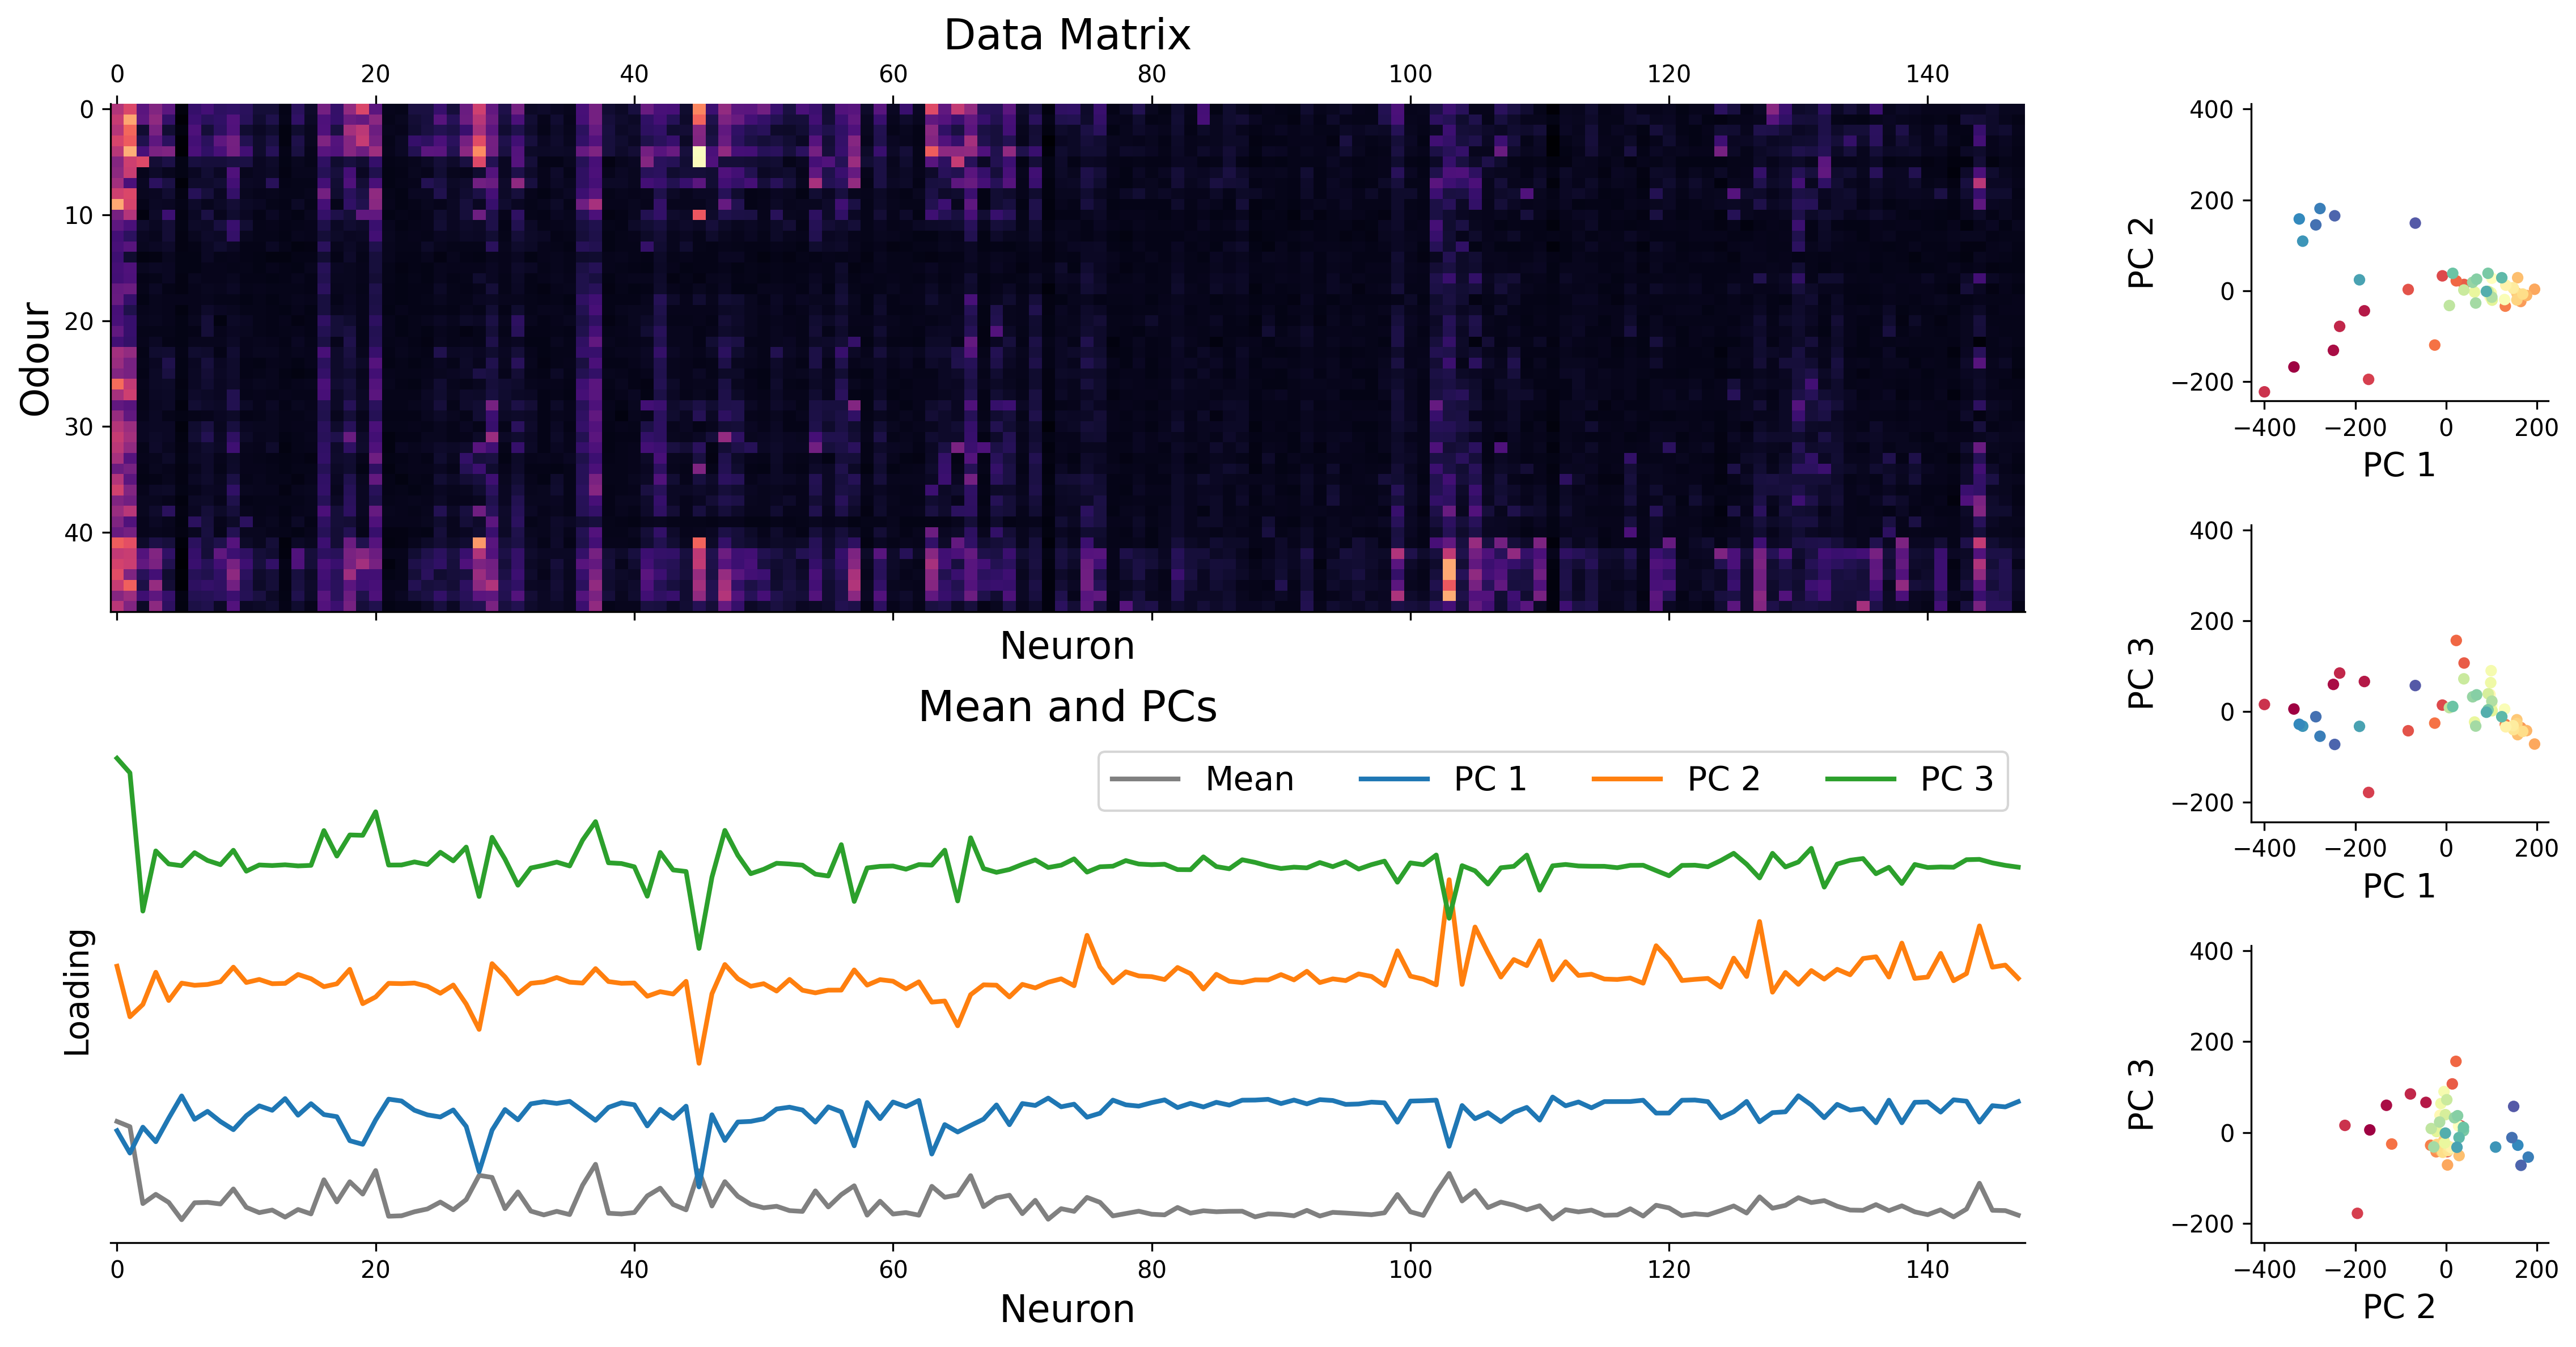
\includegraphics[width=1.0\textwidth]{figures/pca_projections_pcs.png}
\end{center}
\end{frame}
\begin{frame}[label={sec:orgd1e8410}]{Measuring dimensionality with Participation Ratio}
\begin{itemize}
\item Variances tell us energy in each direction
\item Use this as a measure of dimensionality
$$ \text{PR} = {(\sum_i s_i)^2 \over \sum_i s_i^2}.$$
\end{itemize}
\begin{center}
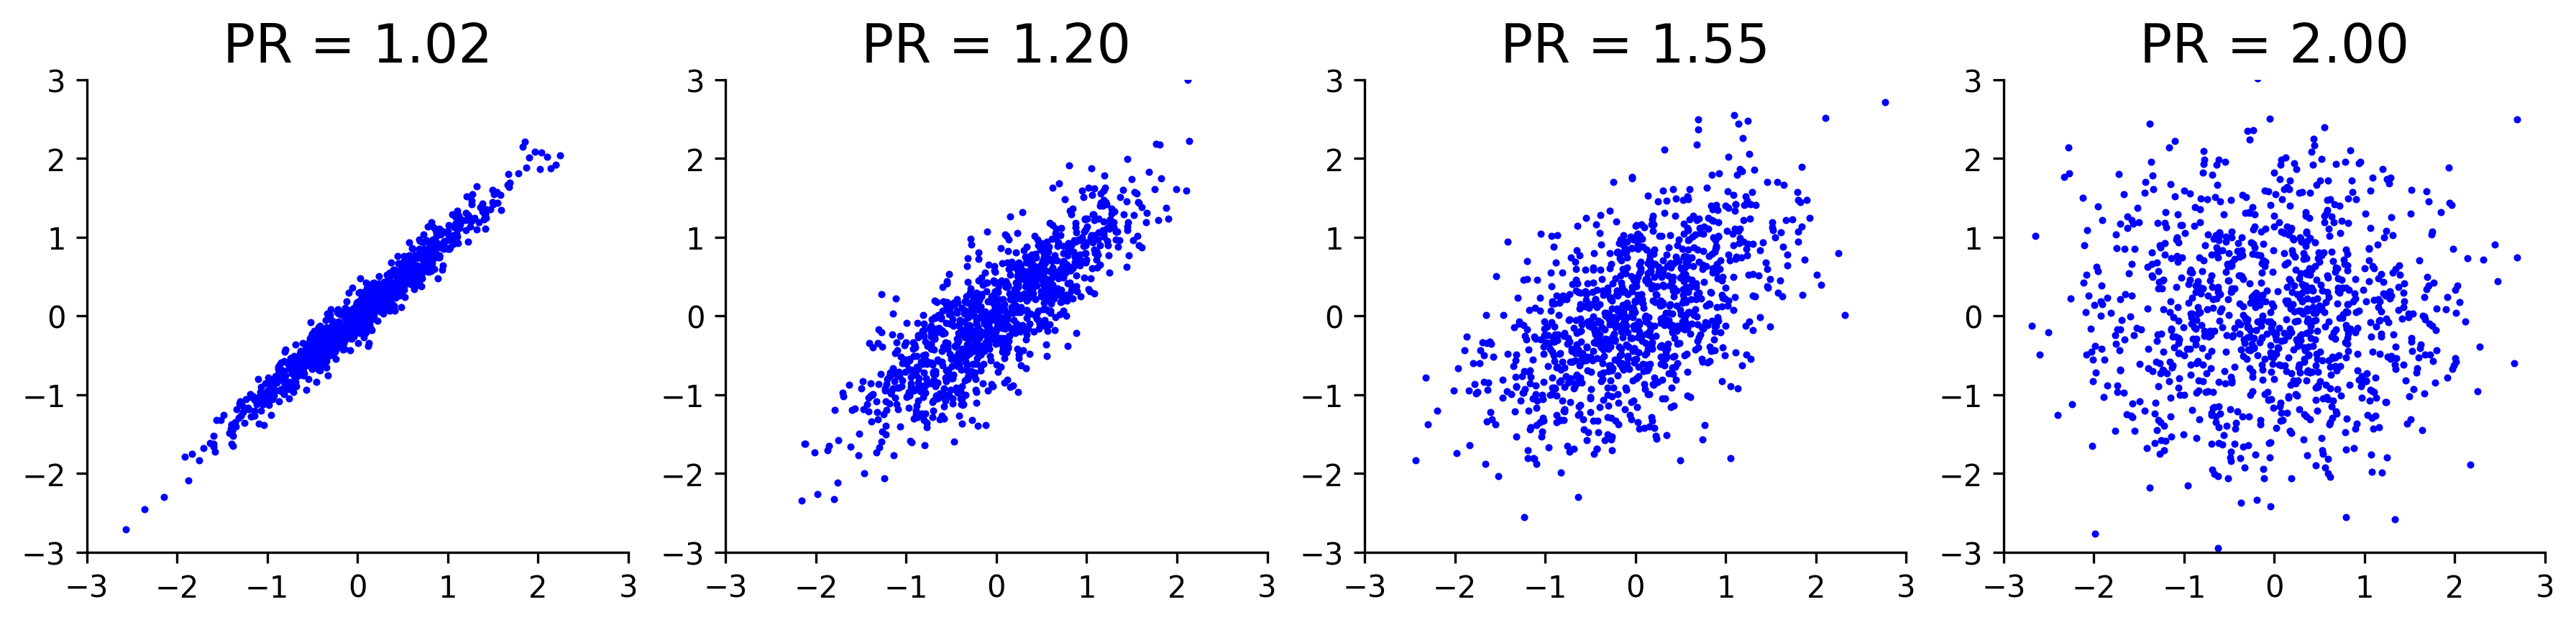
\includegraphics[width=1.0\textwidth]{figures/participation_ratio.png}
\end{center}  
\end{frame}
\begin{frame}[label={sec:org6cb6738}]{Approximation/Denoising with PCA}
\begin{itemize}
\item Approximate using first \(K\) projections
\begin{align*}
\xx &\approx \underbrace{\sum_{i=1}^K (\xx^T \vv_i) \vv_i}_{\text{Exact}} + \underbrace{\sum_{i=K+1}^D (\overline{\xx}^T \vv_i) \vv_i}_{\text{Approximation}}.\\
&\approx  \overline{\xx} + \sum_{i=1}^K (\xx - \overline{\xx})^T \vv_i \vv_i
\end{align*}
\end{itemize}
\begin{figure}[htbp]
\centering
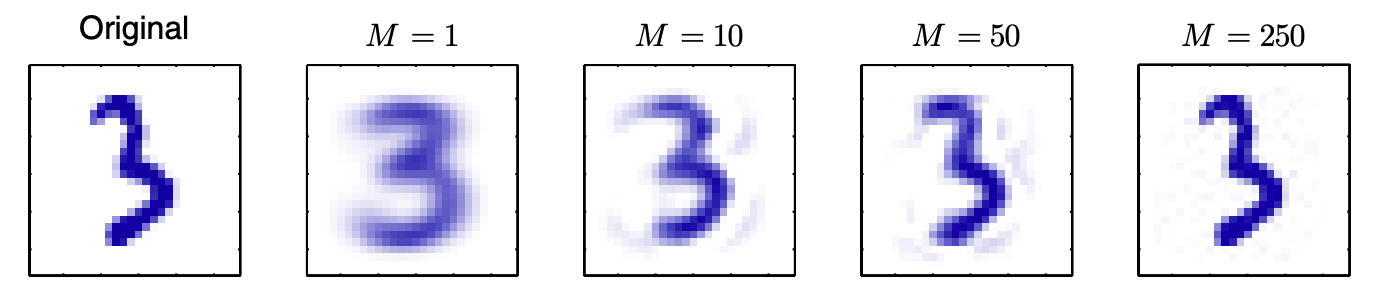
\includegraphics[width=1.0\textwidth]{figures/bishop_approx.png}
\caption{Approximating digits data using PCA (Bishop Fig 12.5)}
\end{figure}
\end{frame}
\begin{frame}[label={sec:orgfe9230c}]{Approximation/Denoising with PCA}
\begin{figure}[htbp]
\centering
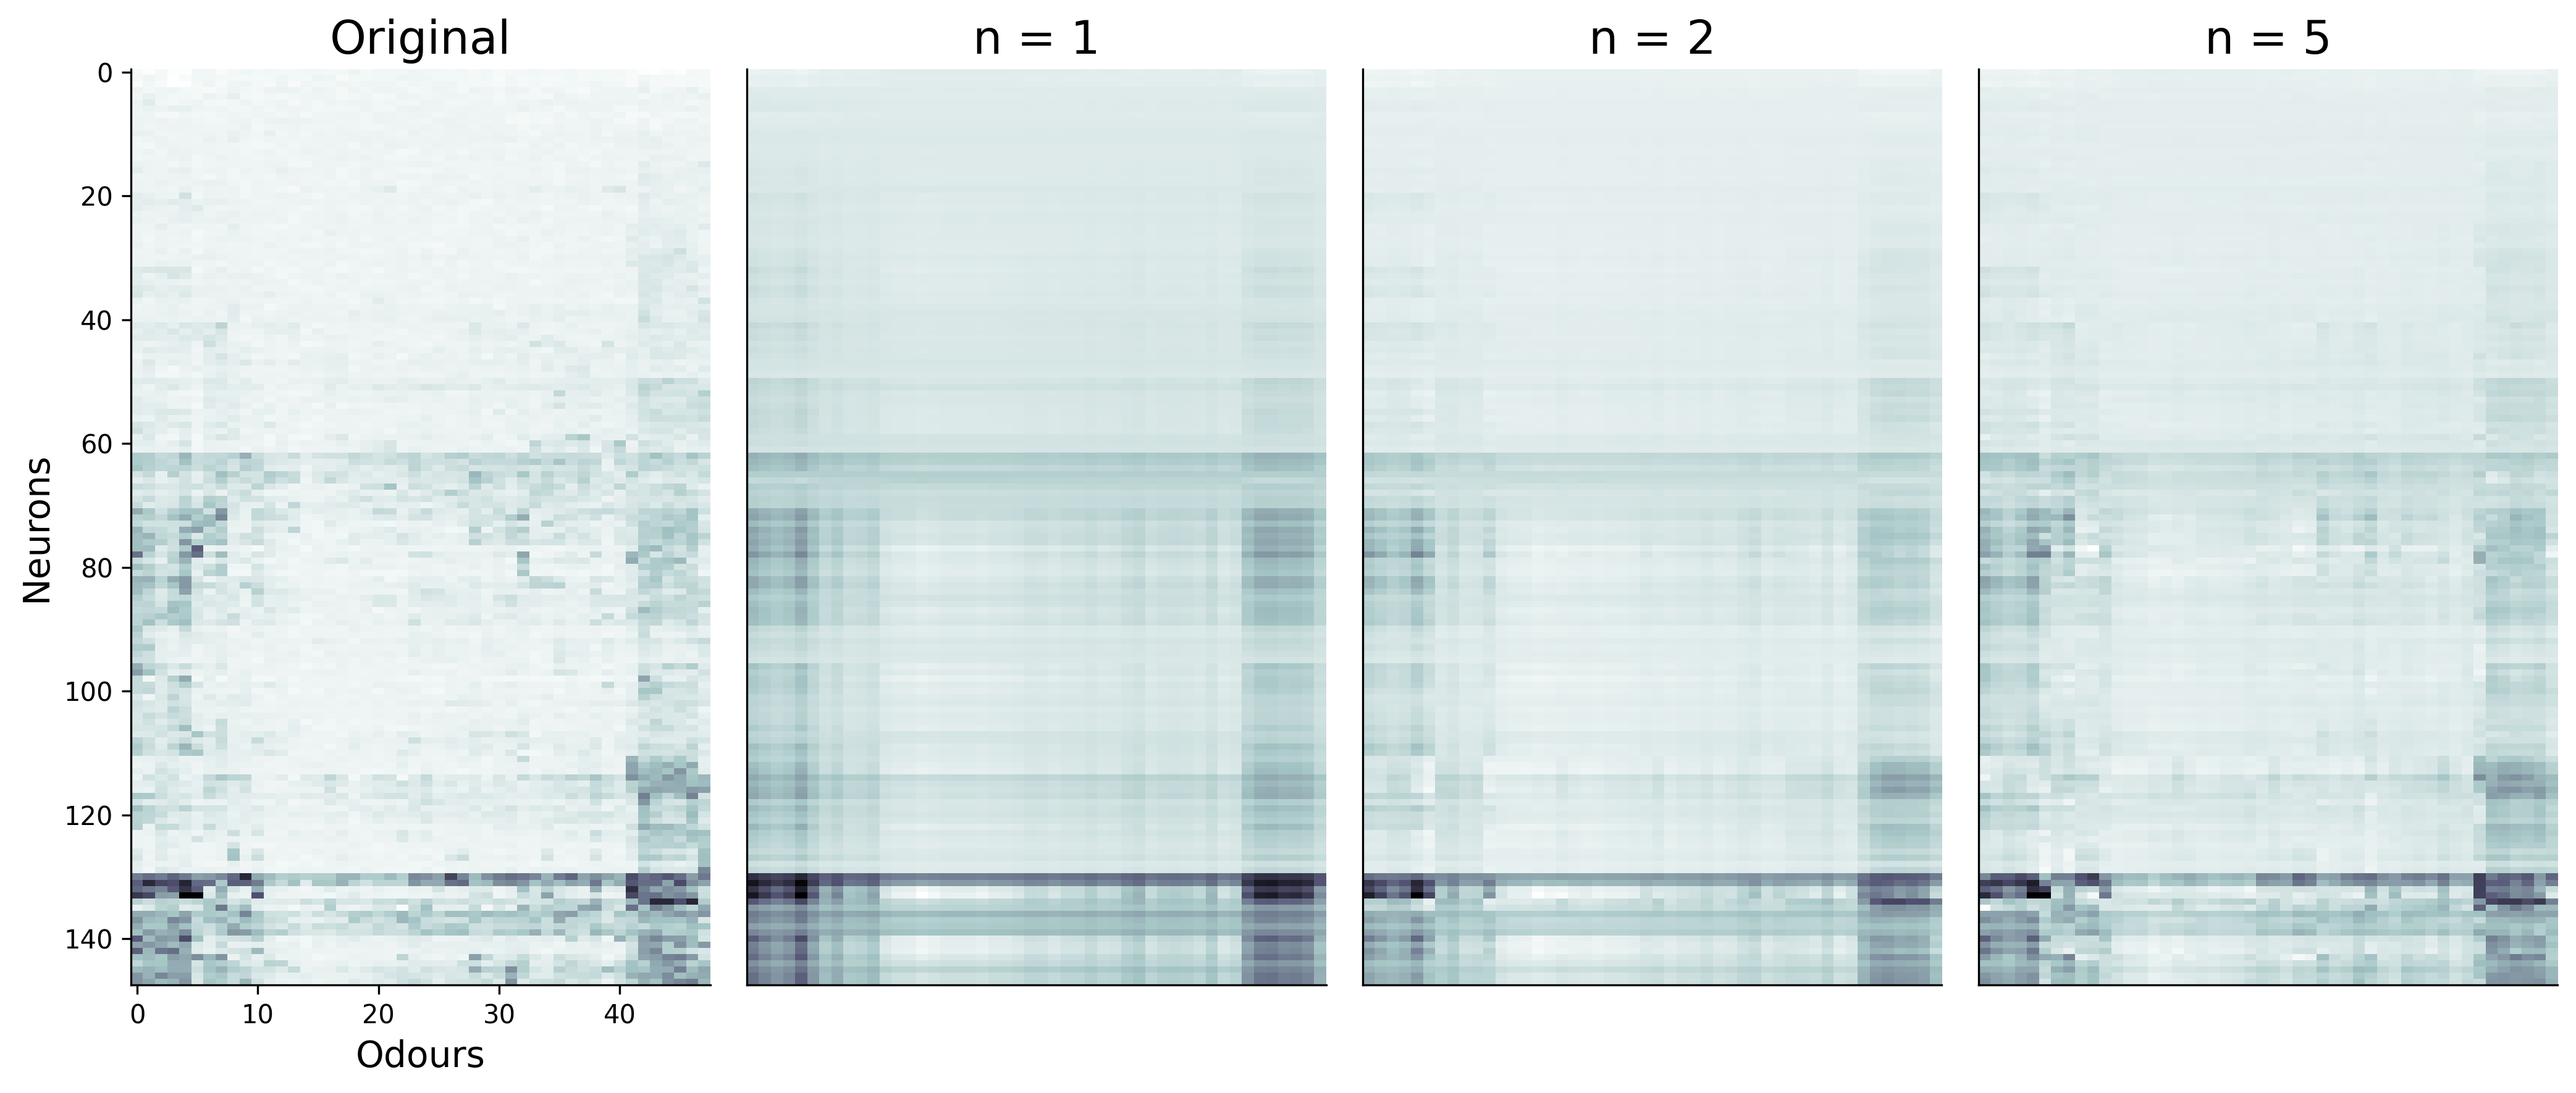
\includegraphics[width=1.0\textwidth]{figures/pca_tobias.png}
\caption{Approximating odour responses using PCA.}
\end{figure}
\end{frame}
\begin{frame}[label={sec:org57938c5}]{How many dimensions to keep?}
\begin{itemize}
\item The singular values tell us how much variance is explained by each dimension.
\item We can use this to decide how many dimensions to keep.
\item \bold{Explained variance} measures the fraction of variance explained by the first \(K\) dimensions:
$$ \text{EV}(K) = { \sum_{i=1}^K s_i \over \sum_{i=1}^D s_i}.$$
\end{itemize}
\begin{figure}[htbp]
\centering
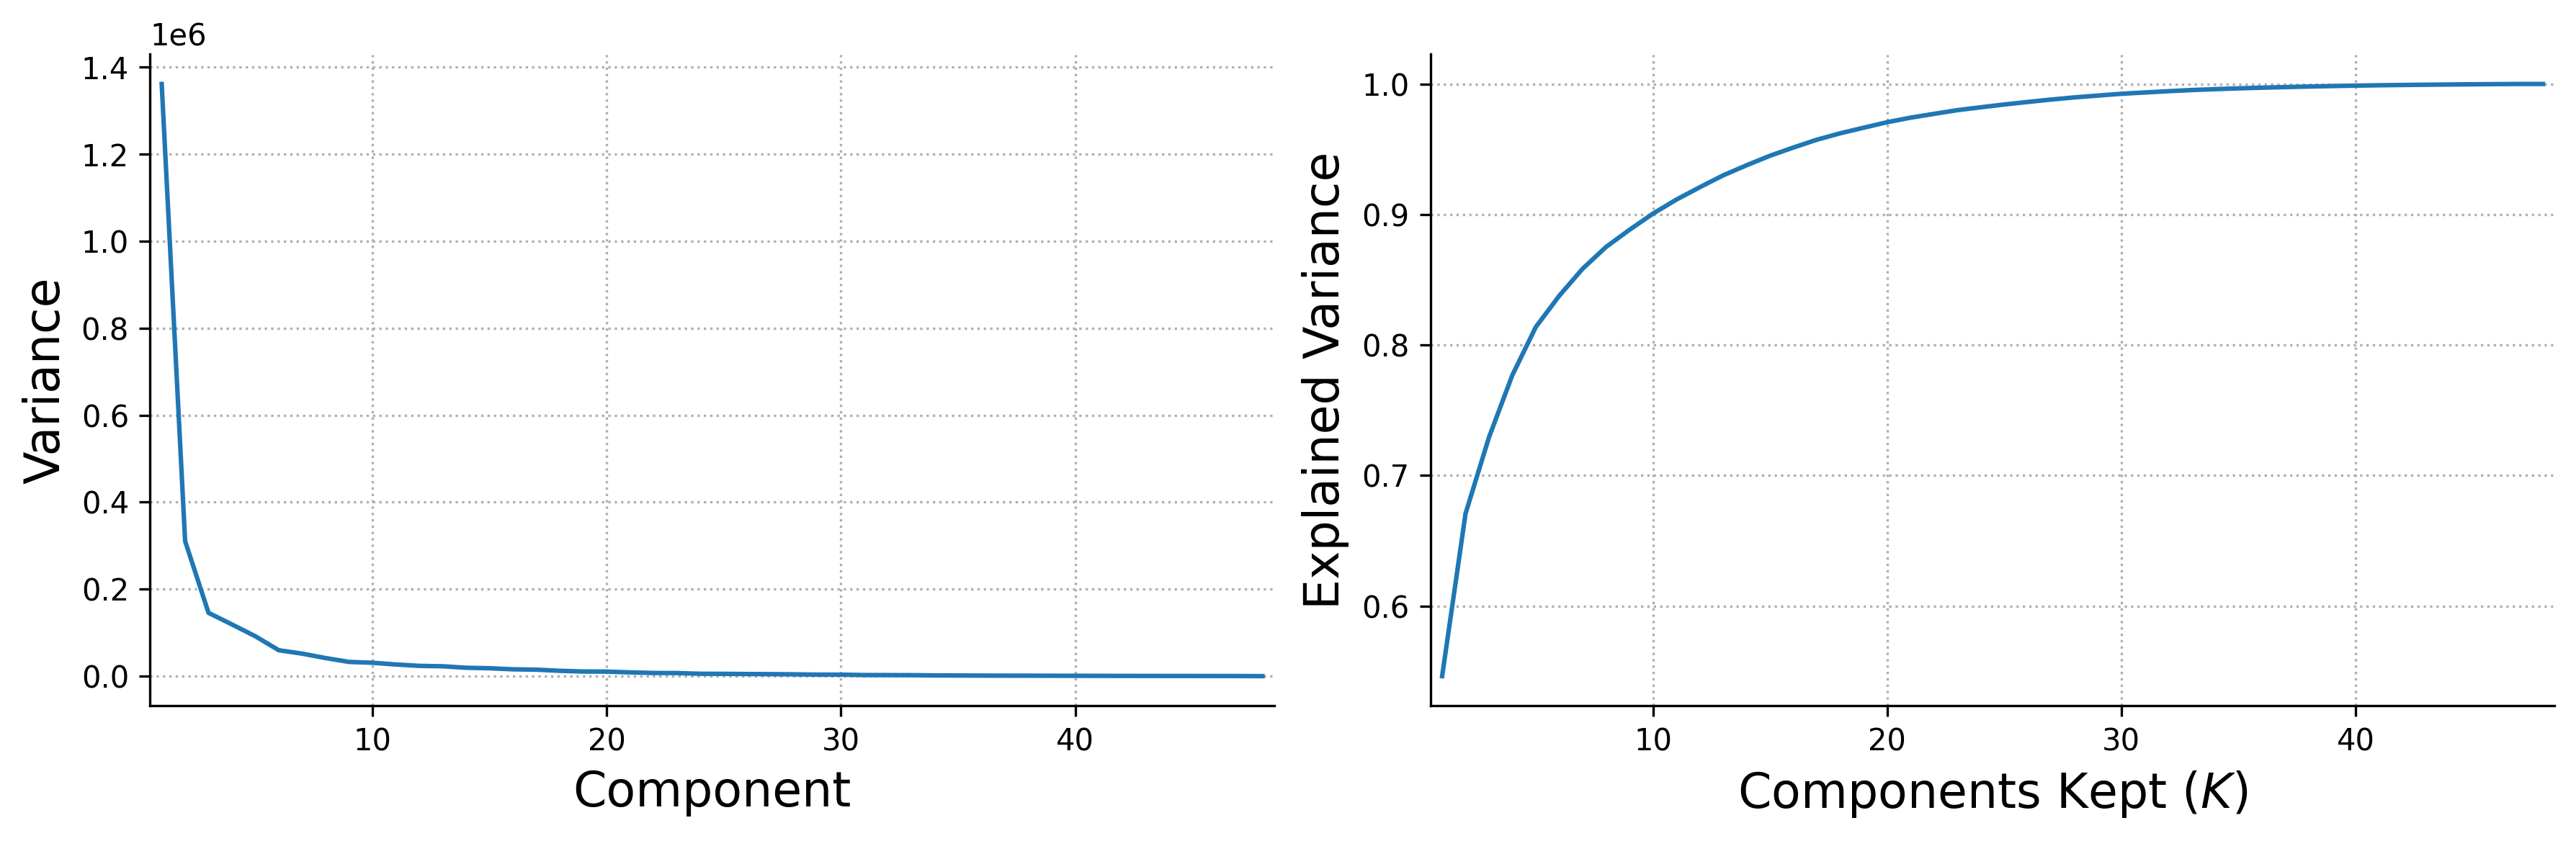
\includegraphics[width=1.0\textwidth]{figures/explained_variance.png}
\caption{Explained variance for odour responses dataset.}
\end{figure}
\end{frame}
\section{Adjacent Approaches}
\label{sec:orga72fa5c}
\begin{frame}[label={sec:org332bf6e}]{Exploiting nonlinearity with Kernel PCA}
\begin{itemize}
\item PCA can be expressed in terms of similarity \(k(\xx,\yy)\) between data points.
\item PCA uses linear similarity \(k(\xx, \yy) = \xx^T \yy\).
\item Kernel PCA generalises this to allow other similarity measures.
\item Nonlinear measures are sometimes appropriate.
\end{itemize}
\begin{figure}[htbp]
\centering
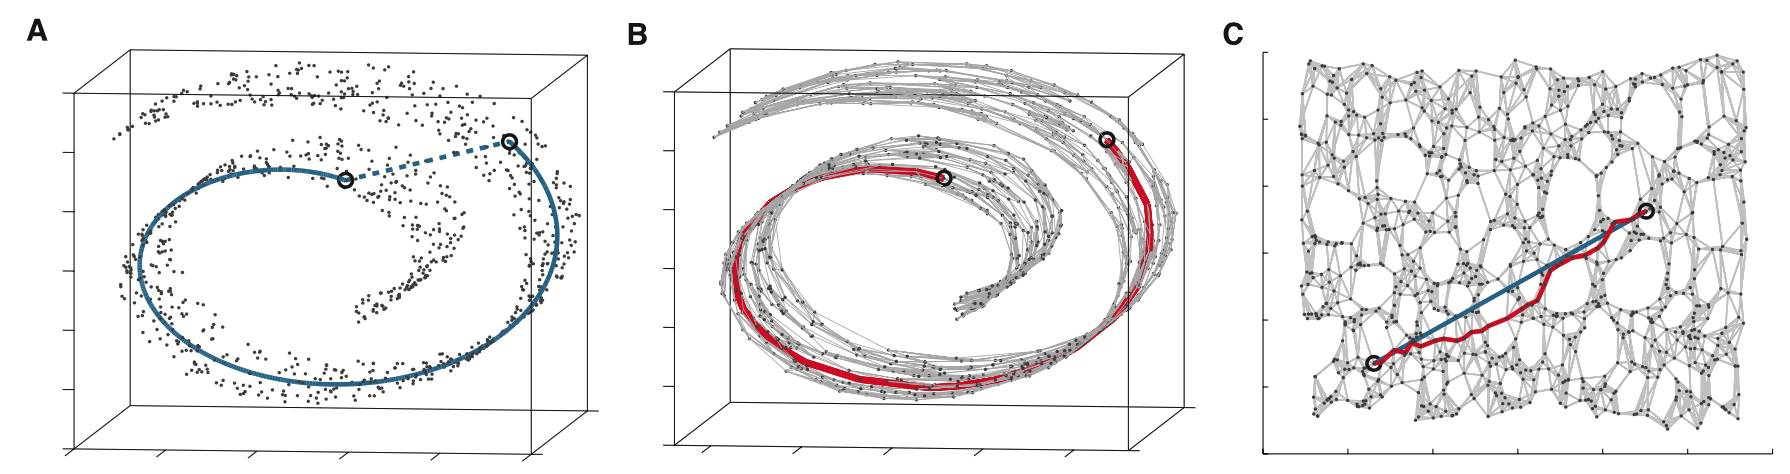
\includegraphics[width=1.0\textwidth]{figures/swiss_roll.png}
\caption{ISOMAP computes similarity as distance on the manifold.}
\end{figure}
\end{frame}
\begin{frame}[label={sec:org99f317b}]{Comparing different datasets with CCA}
\begin{itemize}
\item PCA finds maximum variance directions in one dataset
\item CCA finds maximum co-variance directions in two datasets
\end{itemize}
\begin{center}
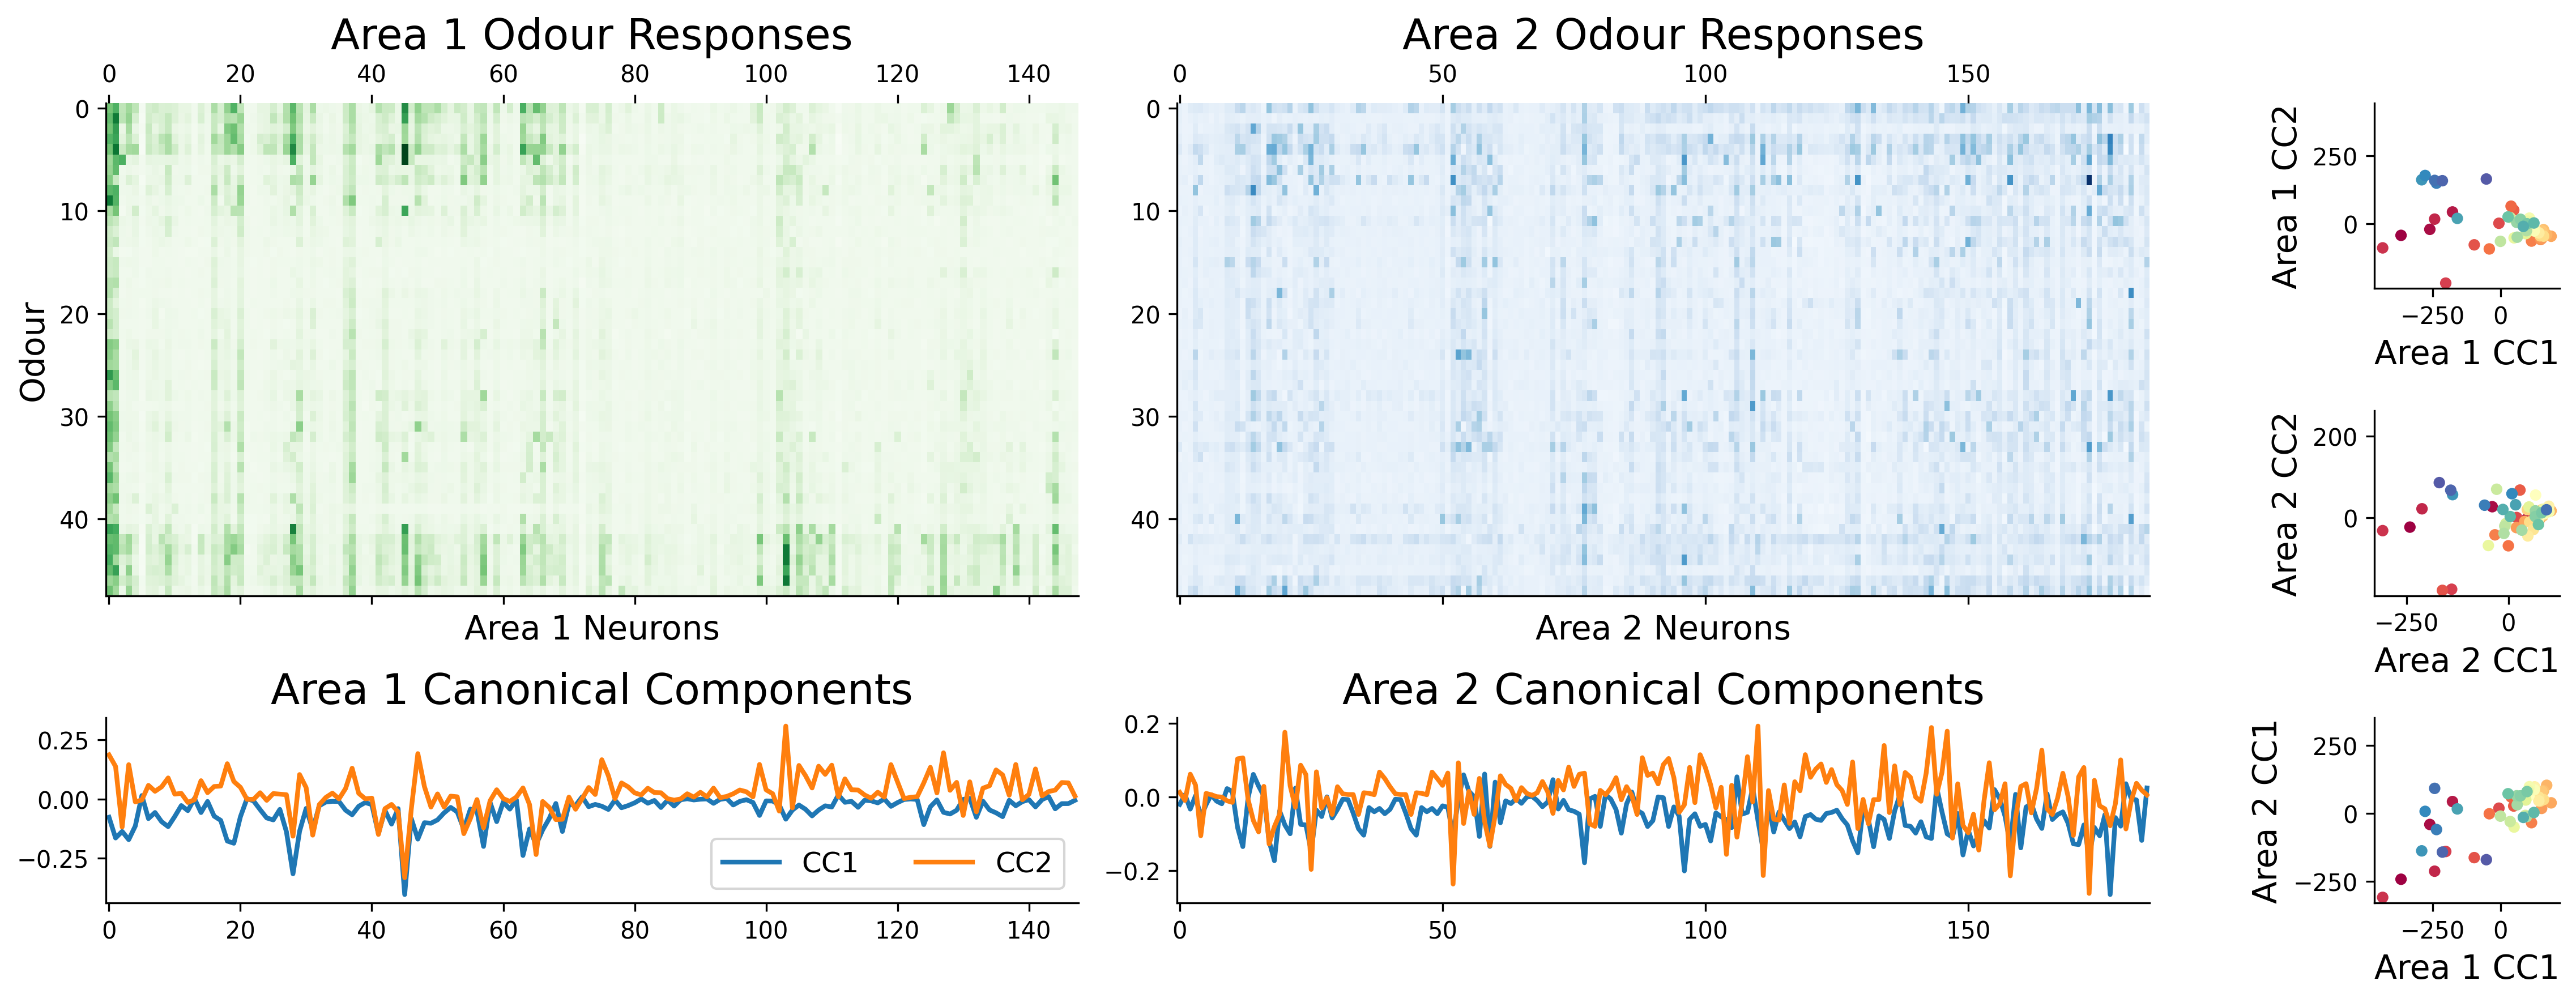
\includegraphics[width=1.0\textwidth]{figures/cca_projections.png}
\end{center}  
\end{frame}
\begin{frame}[label={sec:orgf00a985}]{Supervised learning with LDA}
\begin{itemize}
\item PCA doesn't care about class labels.
\item Maximum variance isn't always best for discrimination.
\item LDA: Finds directions that best discriminate data.
\end{itemize}
\begin{figure}[htbp]
\centering
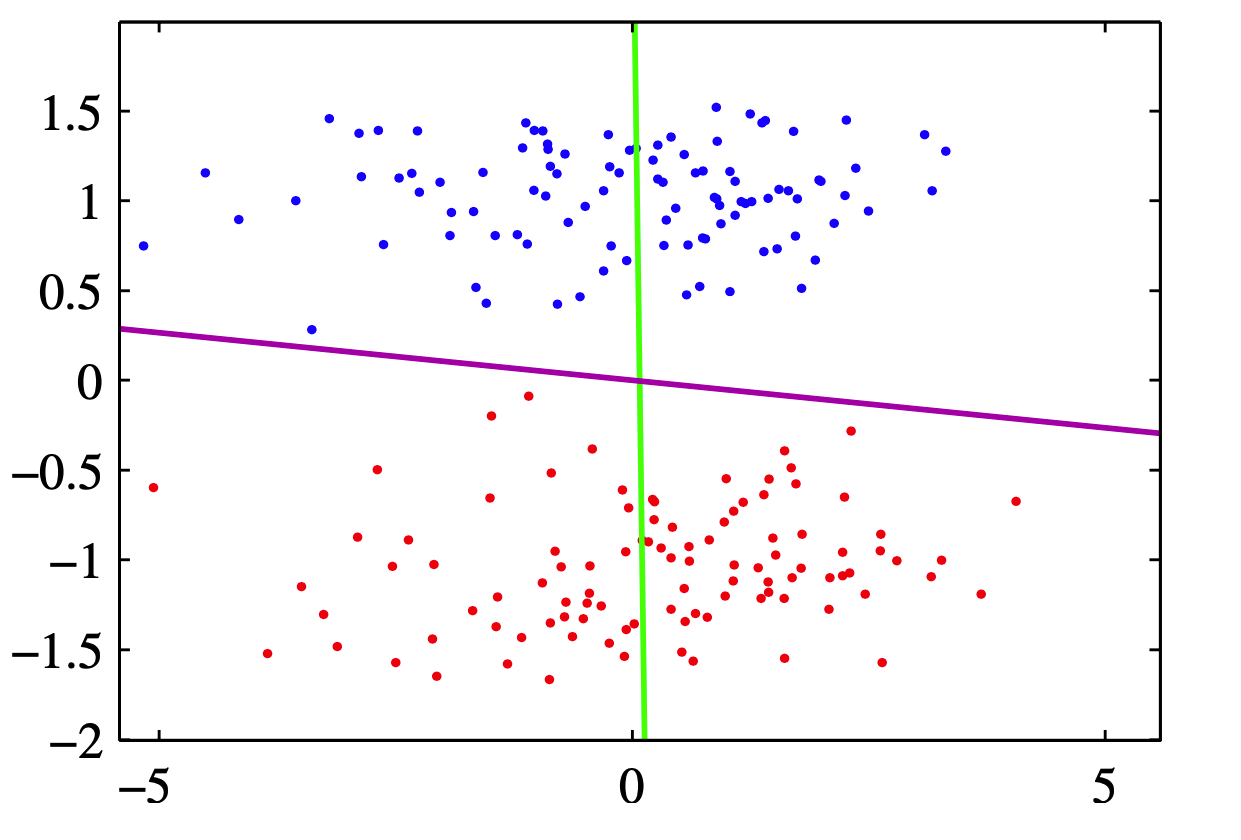
\includegraphics[width=0.7\textwidth]{figures/pca_lda.png}
\caption{(Bishop Fig. 12.7) The first PC isn't always best for discrimination.}
\end{figure}]]
\end{frame}
\section{Summary}
\label{sec:org1d9ee37}
\begin{frame}[label={sec:org970a90c}]{Summary}
\begin{itemize}
\item Neural data arrive in single neuron coordinates.
\item Other coordinates may be more informative about the data.
\item PCA finds coordinates that capture most variance.
\item Can be found through SVD.
\item Can be used for dimensionality reduction and visualization.
\item Can be used for approximation and denoising.
\item Many extensions, including Kernel PCA, CCA, LDA.
\end{itemize}
\end{frame}
\section{Thanks for listening!}
\label{sec:orgebdfa63}
\end{document}